\subsection{Scalability and performance of data centers}

\subsubsection{Evaluate system quality}

System quality information is critical from a cost and performance perspective. In this context, \dquotes{\emph{performance}} means the \textbf{overall effectiveness of a computer system in terms of throughput}, \textbf{response time}, and \textbf{availability}.

\begin{flushleft}
	\textcolor{Green3}{\faIcon{question-circle} \textbf{So how do we evaluate system quality?}}
\end{flushleft}
There are generally two approaches:
\begin{itemize}
	\item \textbf{Intuition and trend extrapolation}. Obviously, those who possess these qualities in sufficient quantity are rare. The pros are speed and flexibility, but the cons are accuracy.
	
	\item \textbf{Experimental evaluation of alternatives}. As pro has excellent accuracy, but as con has laborious and flexible.
\end{itemize}
The techniques are represented in the following figure.

\begin{figure}[!htp]
	\centering
	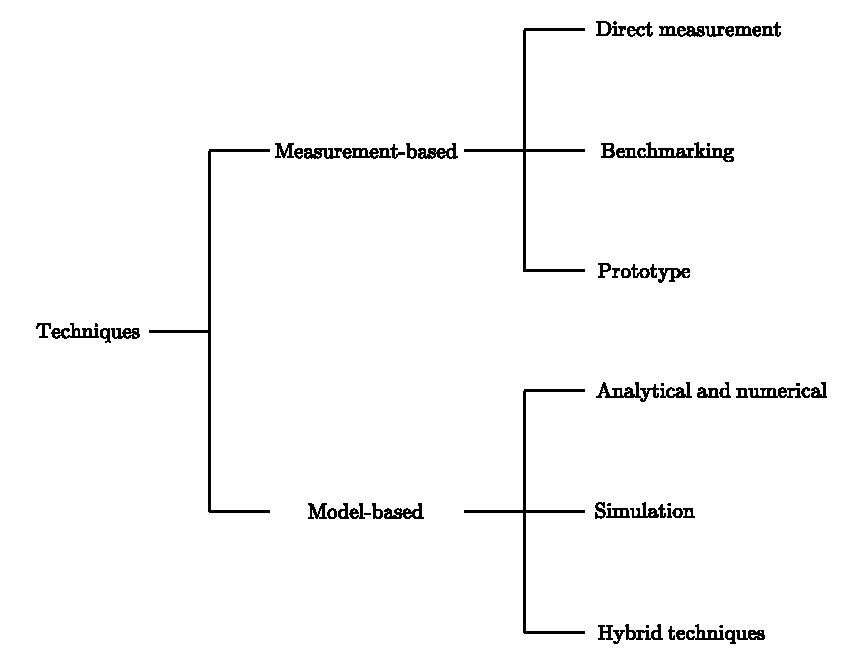
\includegraphics[width=\textwidth]{img/quality-evaluation.pdf}
	\caption{Quality Evaluation techniques.}
	\label{fig: Quality Evaluation techniques}
\end{figure}

\noindent
The most common and useful solution to evaluate system quality is \textbf{model-based approach}. The systems are complex, so it is useful to create an \textbf{abstraction of the systems called models}. The model-based are divided into three groups:
\begin{itemize}
	\item \definition{Analytical and numerical techniques} are based on the \textbf{application of mathematical techniques}, which usually exploit results coming from the theory of probability and stochastic process.
	\begin{flushleft}
		\textcolor{Green3}{\faIcon{check-circle} \textbf{Advantages}}
	\end{flushleft}
	\begin{itemize}
		\item Most \textbf{efficient}.
		\item \textbf{Accurate}.
	\end{itemize}
	\begin{flushleft}
		\textcolor{Red2}{\faIcon{thumbs-down} \textbf{Disadvantages}}
	\end{flushleft}
	\begin{itemize}
		\item \textbf{Available} only in very \textbf{limited cases}.
	\end{itemize}
	
	\item \definition{Simulation techniques} are based on the \textbf{reproduction of traces of the model}.
	\begin{flushleft}
		\textcolor{Green3}{\faIcon{check-circle} \textbf{Advantages}}
	\end{flushleft}
	\begin{itemize}
		\item Most \textbf{general}.
	\end{itemize}
	\begin{flushleft}
		\textcolor{Red2}{\faIcon{thumbs-down} \textbf{Disadvantages}}
	\end{flushleft}
	\begin{itemize}
		\item May be \textbf{less accurate}, especially when considering cases where rare events may occur.
		\item \textbf{Solution time} can also be \textbf{very long} if high accuracy is desired.
	\end{itemize}
	
	\item \definition{Hybrid techniques} \textbf{combine analytical/numerical methods with simulation}.
\end{itemize}

\newpage

\subsubsection{Queueing Networks}\label{subsubsection: Queueing Networks}

\paragraph{Definition}

\definition{Queueing Network Modeling} is a particular approach to computer system modeling in which the \textbf{computer system is represented as a network of queues}. A \emph{network of queues} is a collection of \textbf{service centers}, which represent system \textbf{resources}, and \textbf{customers}, which represent \textbf{users} or \textbf{transactions}.\cite{lazowska1984quantitative}

\highspace
Some \example{examples} of queues in computer systems are:
\begin{itemize}
	\item CPU uses a time-sharing scheduler.
	
	\item A disk serves a queue of requests waiting to read or write blocks.
	
	\item A router on a network serves a queue of packets waiting to be routed.
	
	\item Databases have lock queues where transactions wait to acquire the lock on a record.
\end{itemize}

\begin{figure}[!htp]
	\centering
	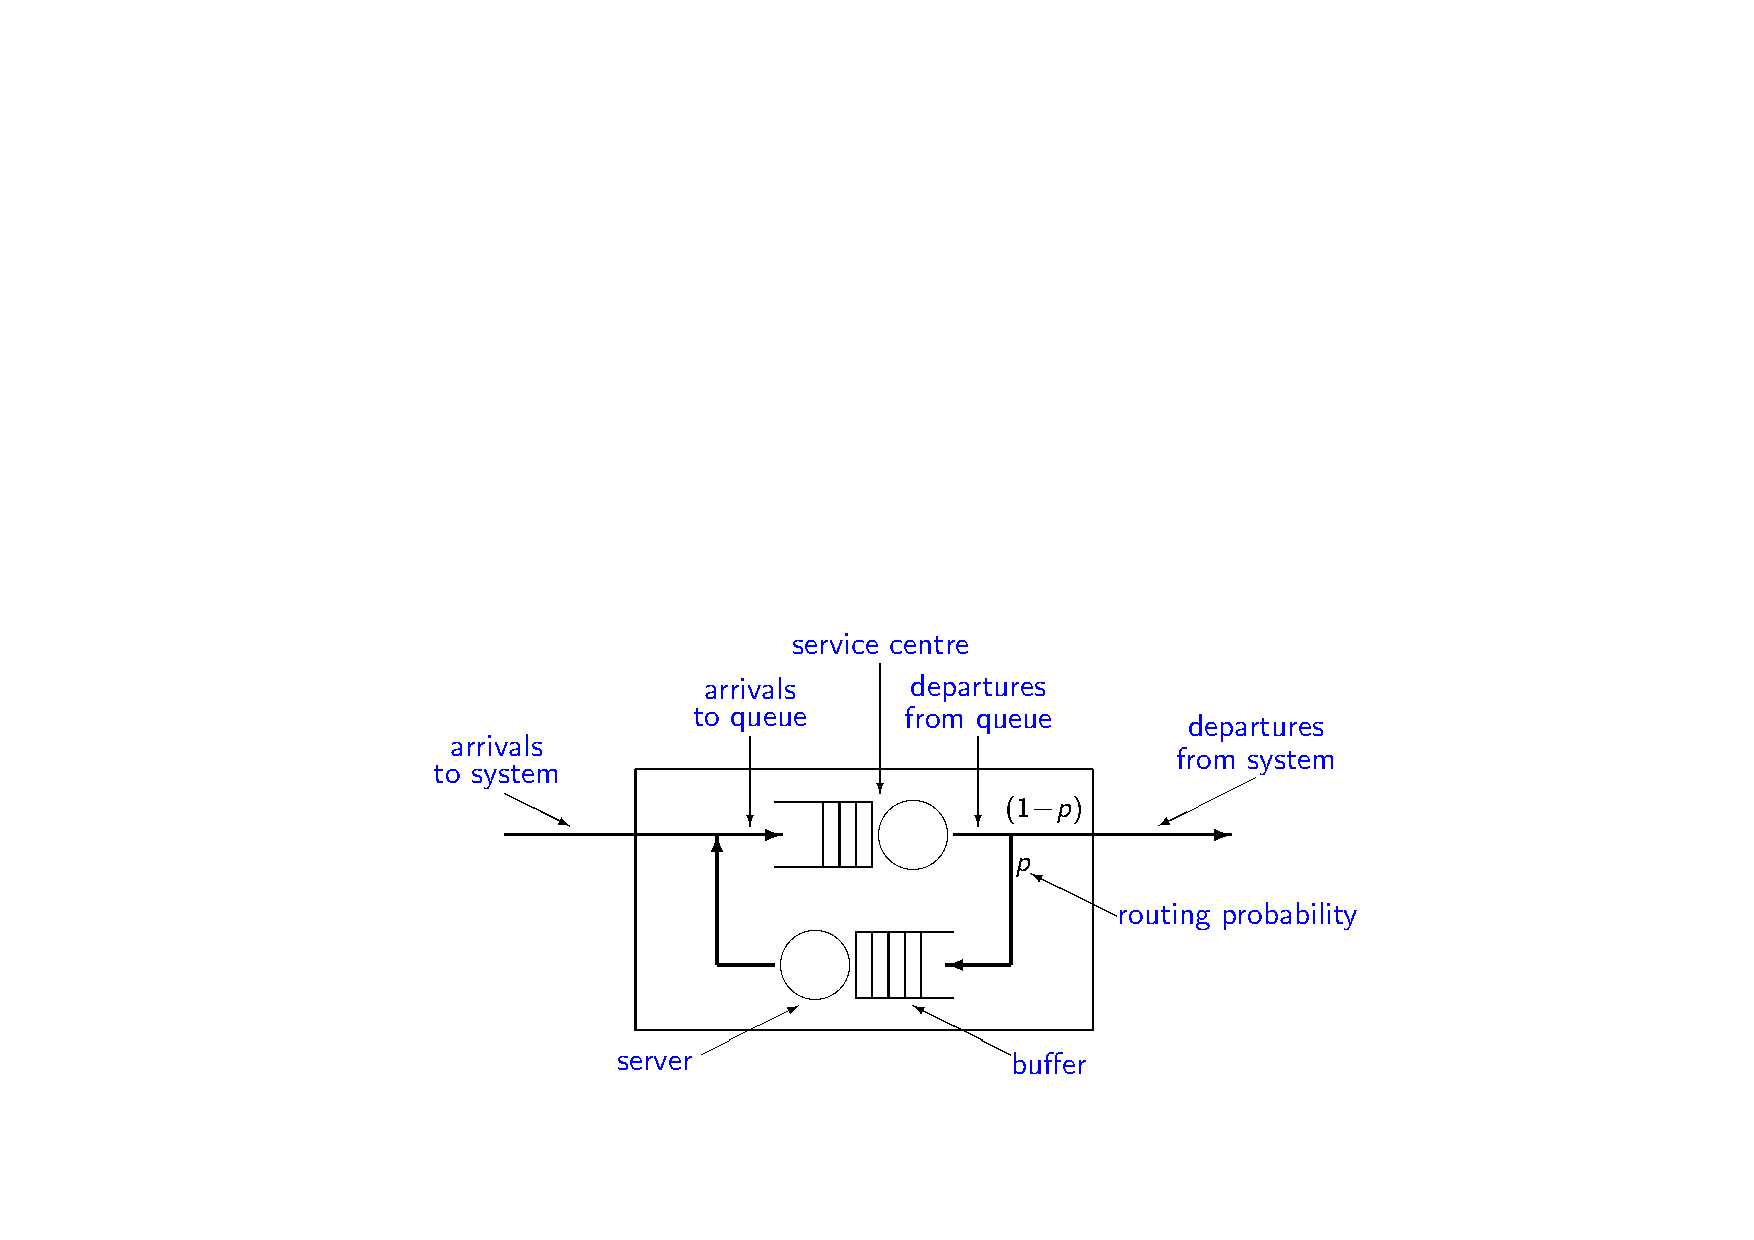
\includegraphics[width=\textwidth]{img/queueing-network-1.pdf}
	\caption{Queueing Network graphical representation.}
\end{figure}

\newpage

\paragraph{Characteristics}

Queueing models are characterized by several aspects:
\begin{itemize}
	\item \textbf{\underline{Arrival}}. Arrivals \textbf{represent orders coming into the system}. They specify \emph{how fast}, \emph{how often}, and \emph{what types of jobs} the \textbf{station will service}. \textbf{Arrivals can come from}:
	\begin{enumerate}
		\item An external source.
		\begin{figure}[!htp]
			\centering
			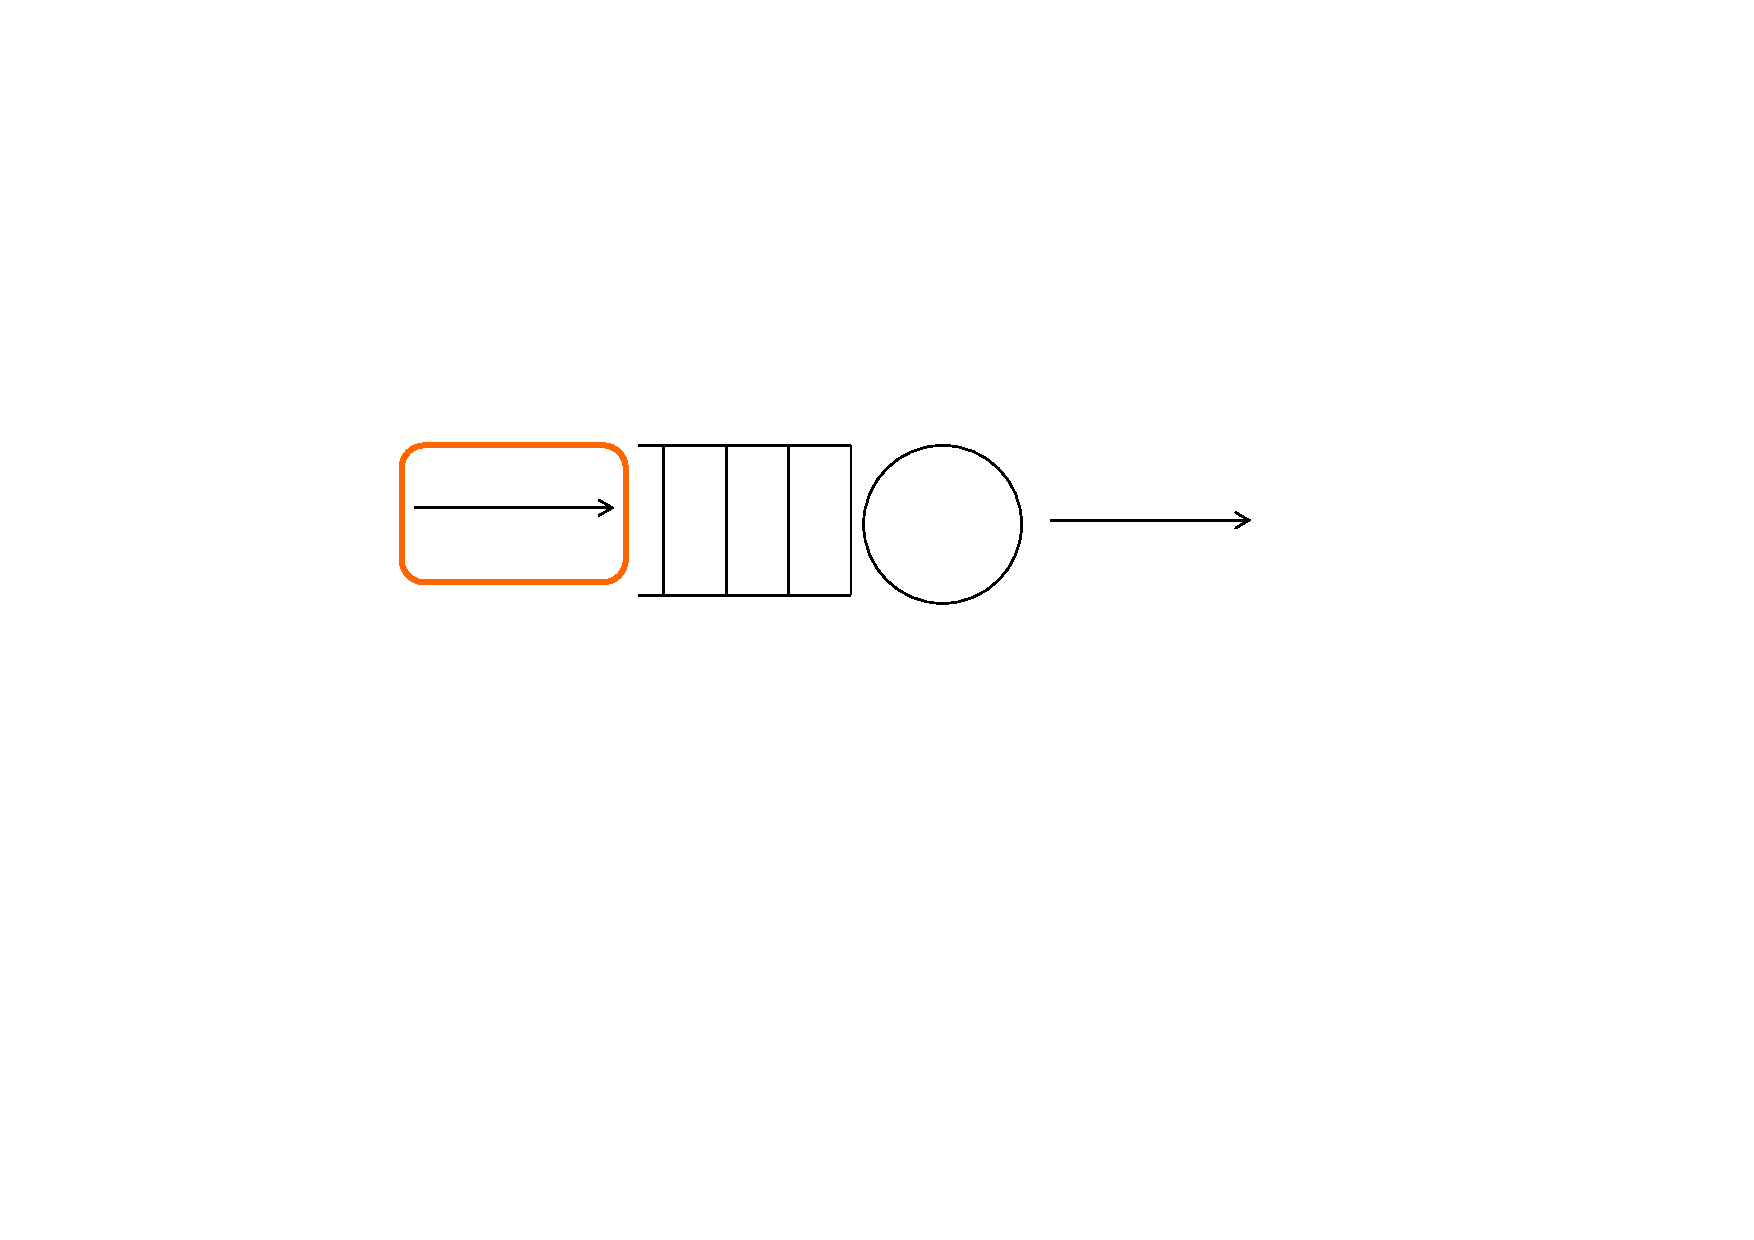
\includegraphics[width=.6\textwidth]{img/queueing-network-2.pdf}
		\end{figure}
		
		\item Another queue.
		\begin{figure}[!htp]
			\centering
			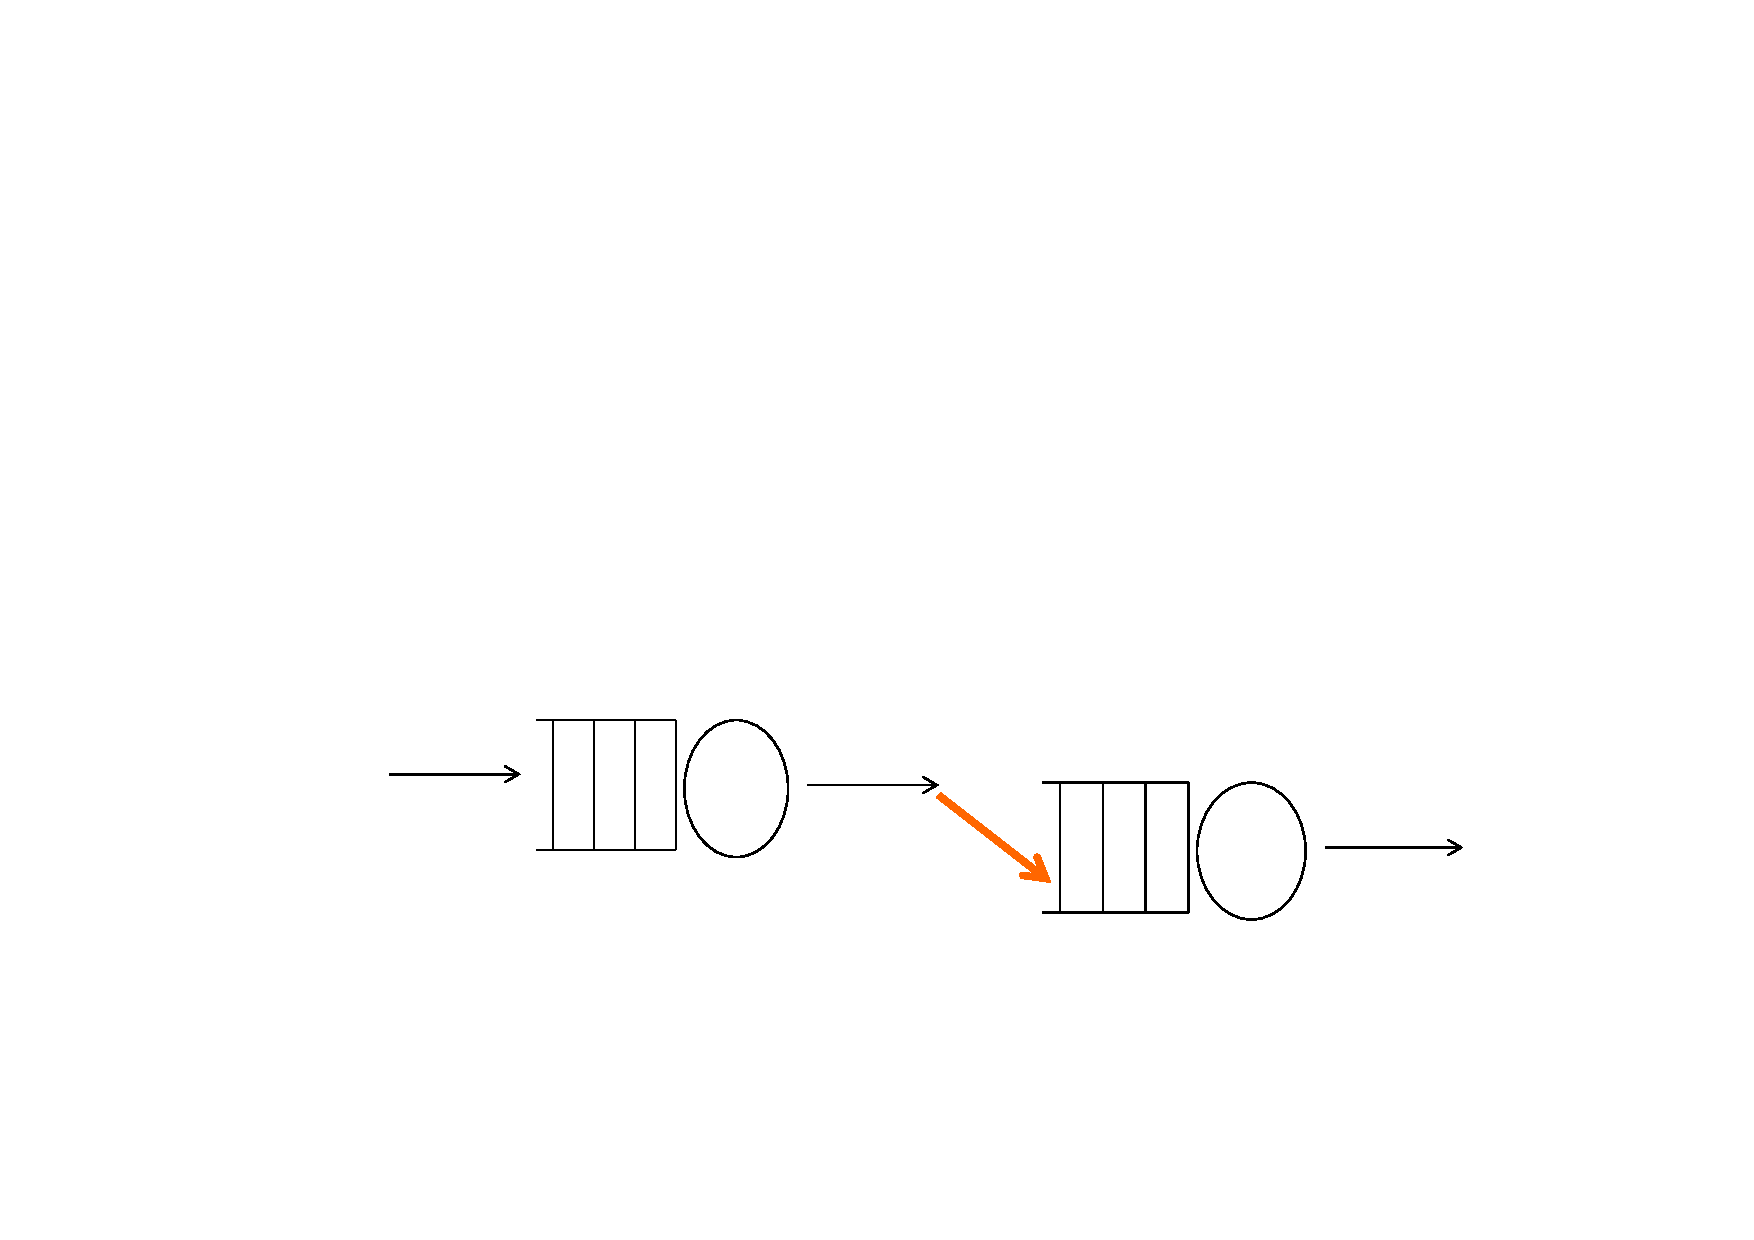
\includegraphics[width=.8\textwidth]{img/queueing-network-3.pdf}
		\end{figure}
		
		\item The same queue, through a loopback arc.
		\begin{figure}[!htp]
			\centering
			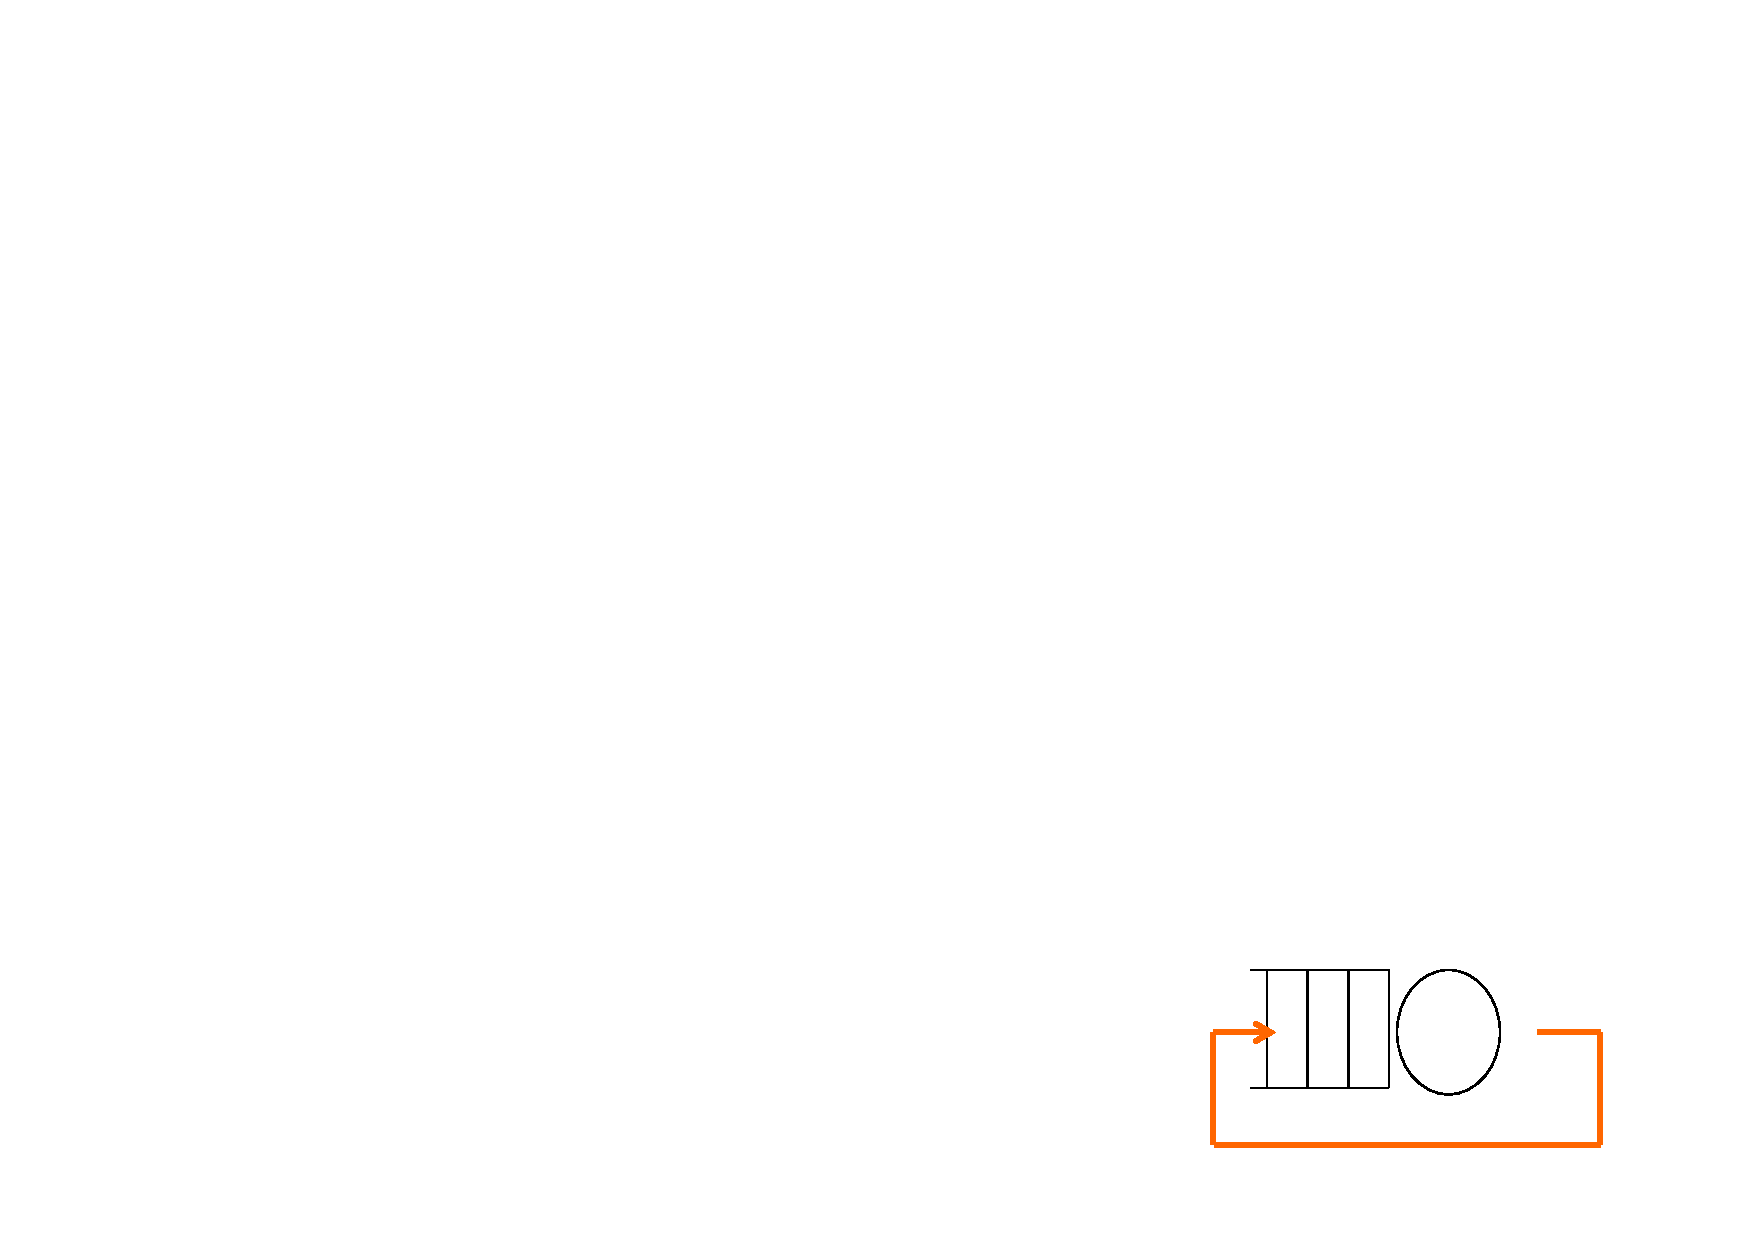
\includegraphics[width=.3\textwidth]{img/queueing-network-4.pdf}
		\end{figure}
	\end{enumerate}
	
	\item \textbf{\underline{Service}}. Service \textbf{represents the time a job spends being served}. The server does the job, but the number of servers can be different:
	\begin{itemize}
		\item \textbf{Single server}. It has the ability to serve \textbf{one client at a time}. \textbf{Waiting customers remain in the buffer} until they are selected for service. Finally, the \textbf{next customer is selected depending on the service discipline}.
		\begin{figure}[!htp]
			\centering
			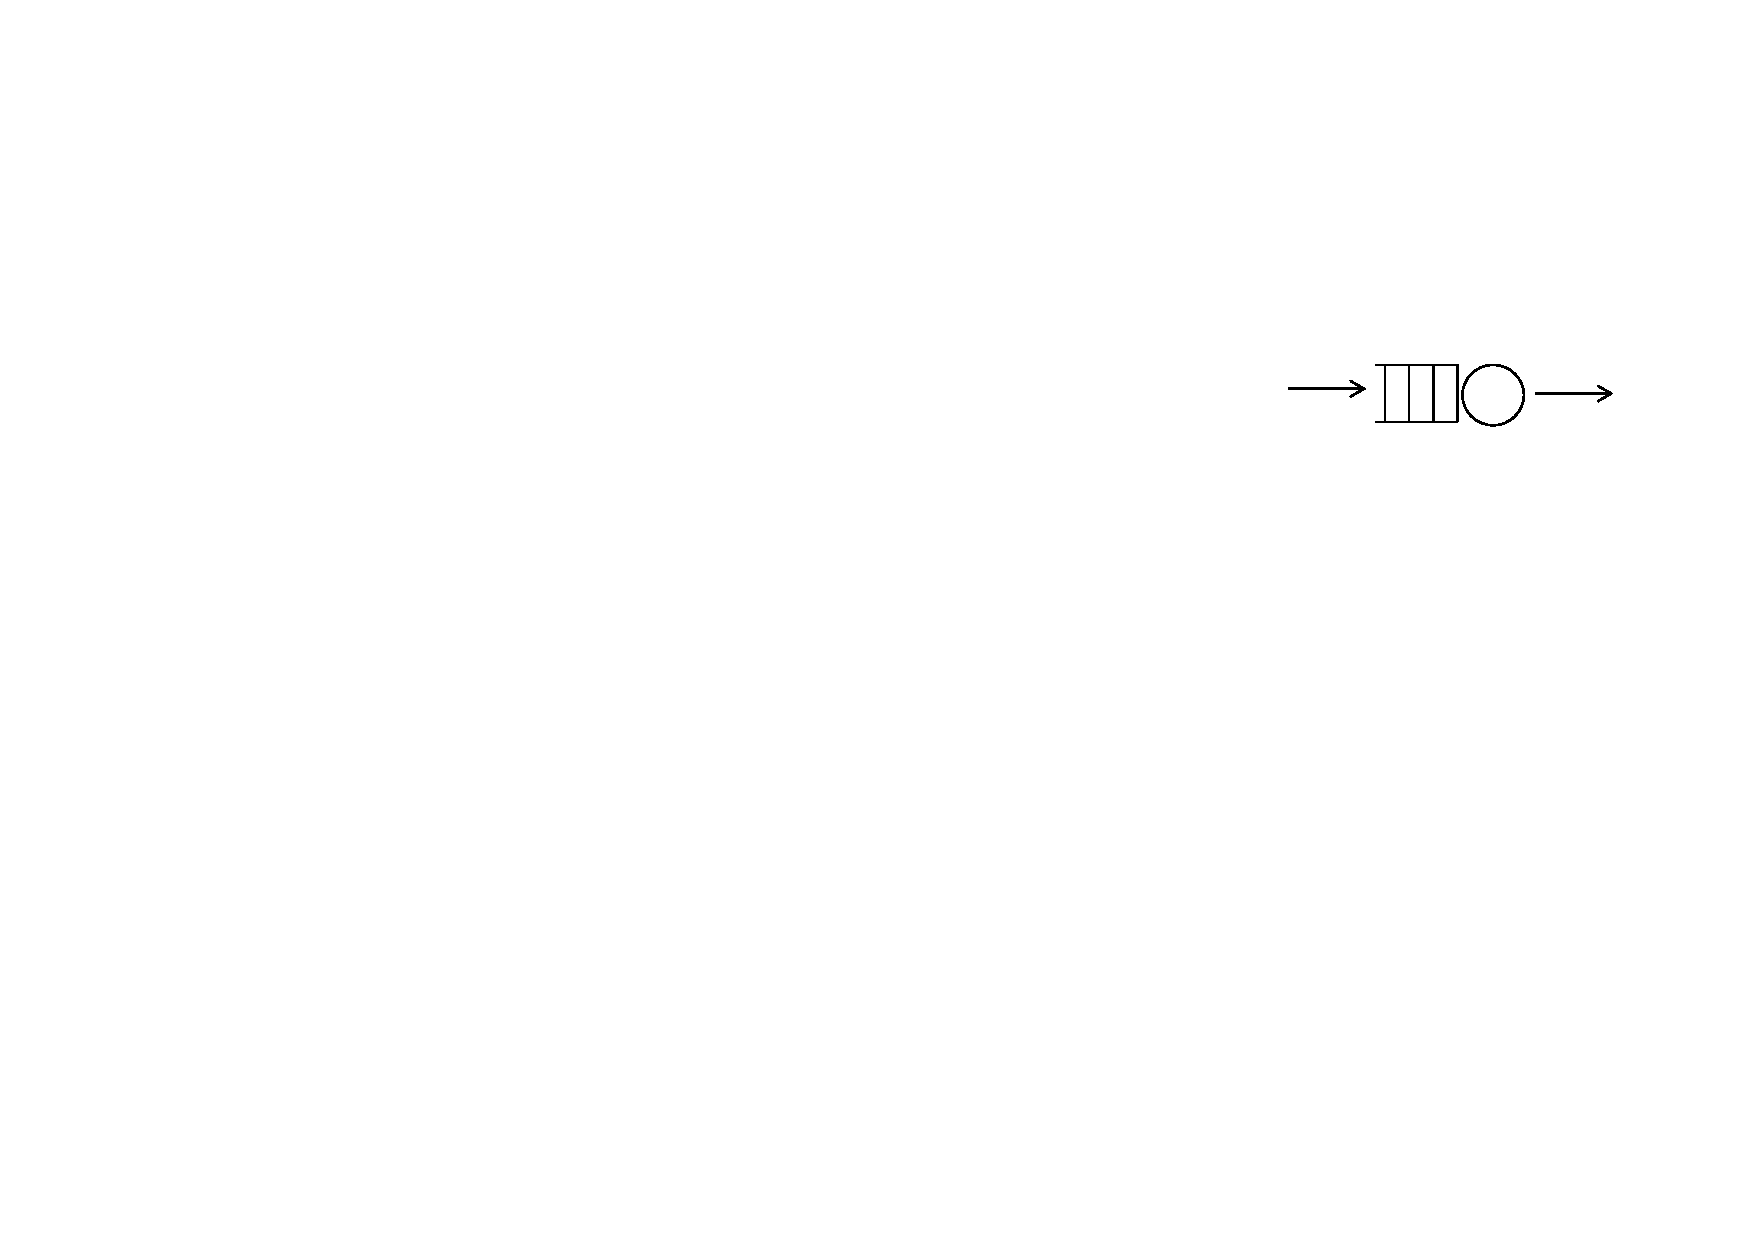
\includegraphics[width=.3\textwidth]{img/queueing-network-5.pdf}
		\end{figure}
		
		\item \textbf{Infinite servers}. There are always at least \textbf{as many servers as there are customers}, and each \textbf{customer can have a dedicated server}. As a consequence, there is \underline{no queuing} (and \underline{no buffer}).
		\begin{figure}[!htp]
			\centering
			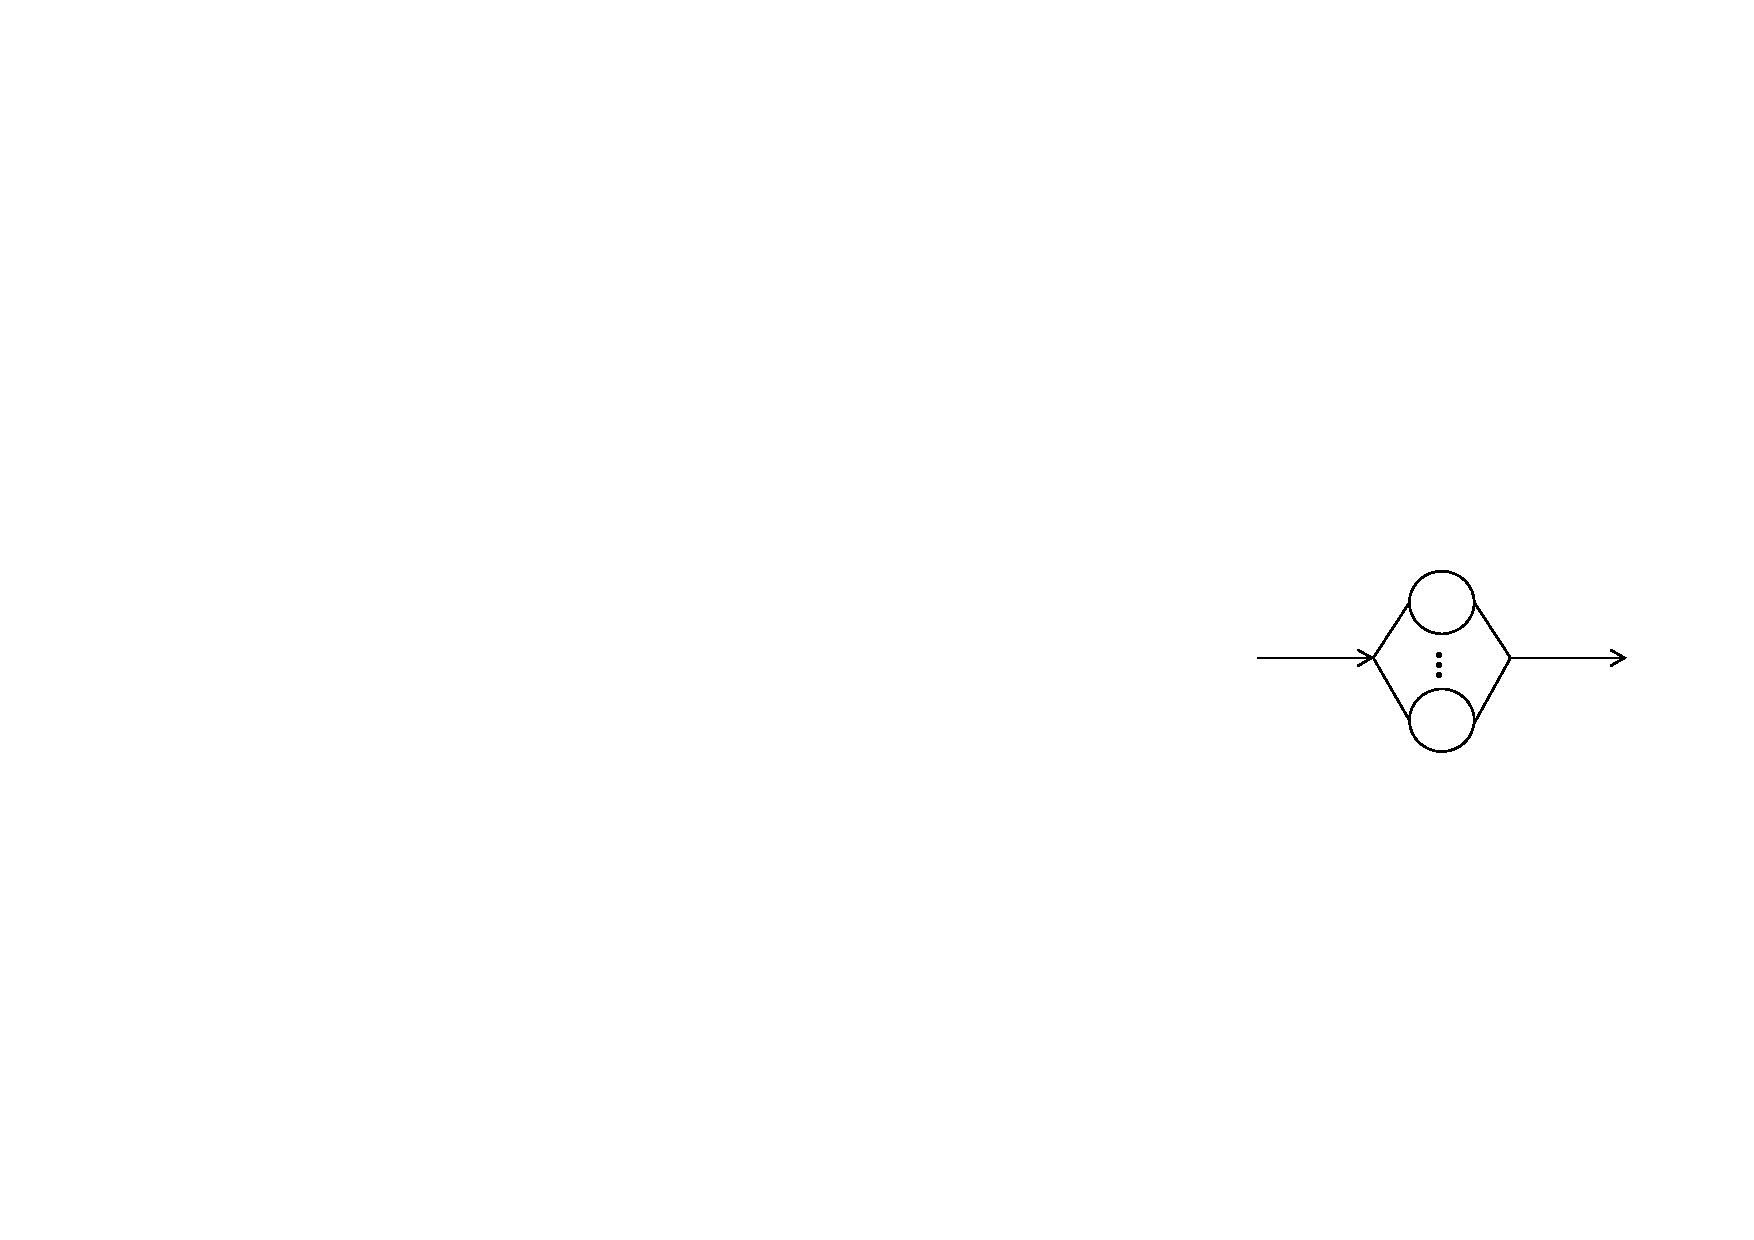
\includegraphics[width=.3\textwidth]{img/queueing-network-6.pdf}
		\end{figure}
		
		\item \textbf{Multiple servers}. There is a \textbf{fixed number of servers} (c in the figure below), each of which can \textbf{serve one customer at a time}. 
		\begin{itemize}
			\item \texttt{Number of customers in the system} $\le$ \texttt{number of servers} $\Rightarrow$ \textbf{no queuing}.
			\item \texttt{Number of customers in the system} $>$ \texttt{number of servers} $\Rightarrow$ the additional \textbf{customers must wait in the buffer}.
		\end{itemize}
		\begin{figure}[!htp]
			\centering
			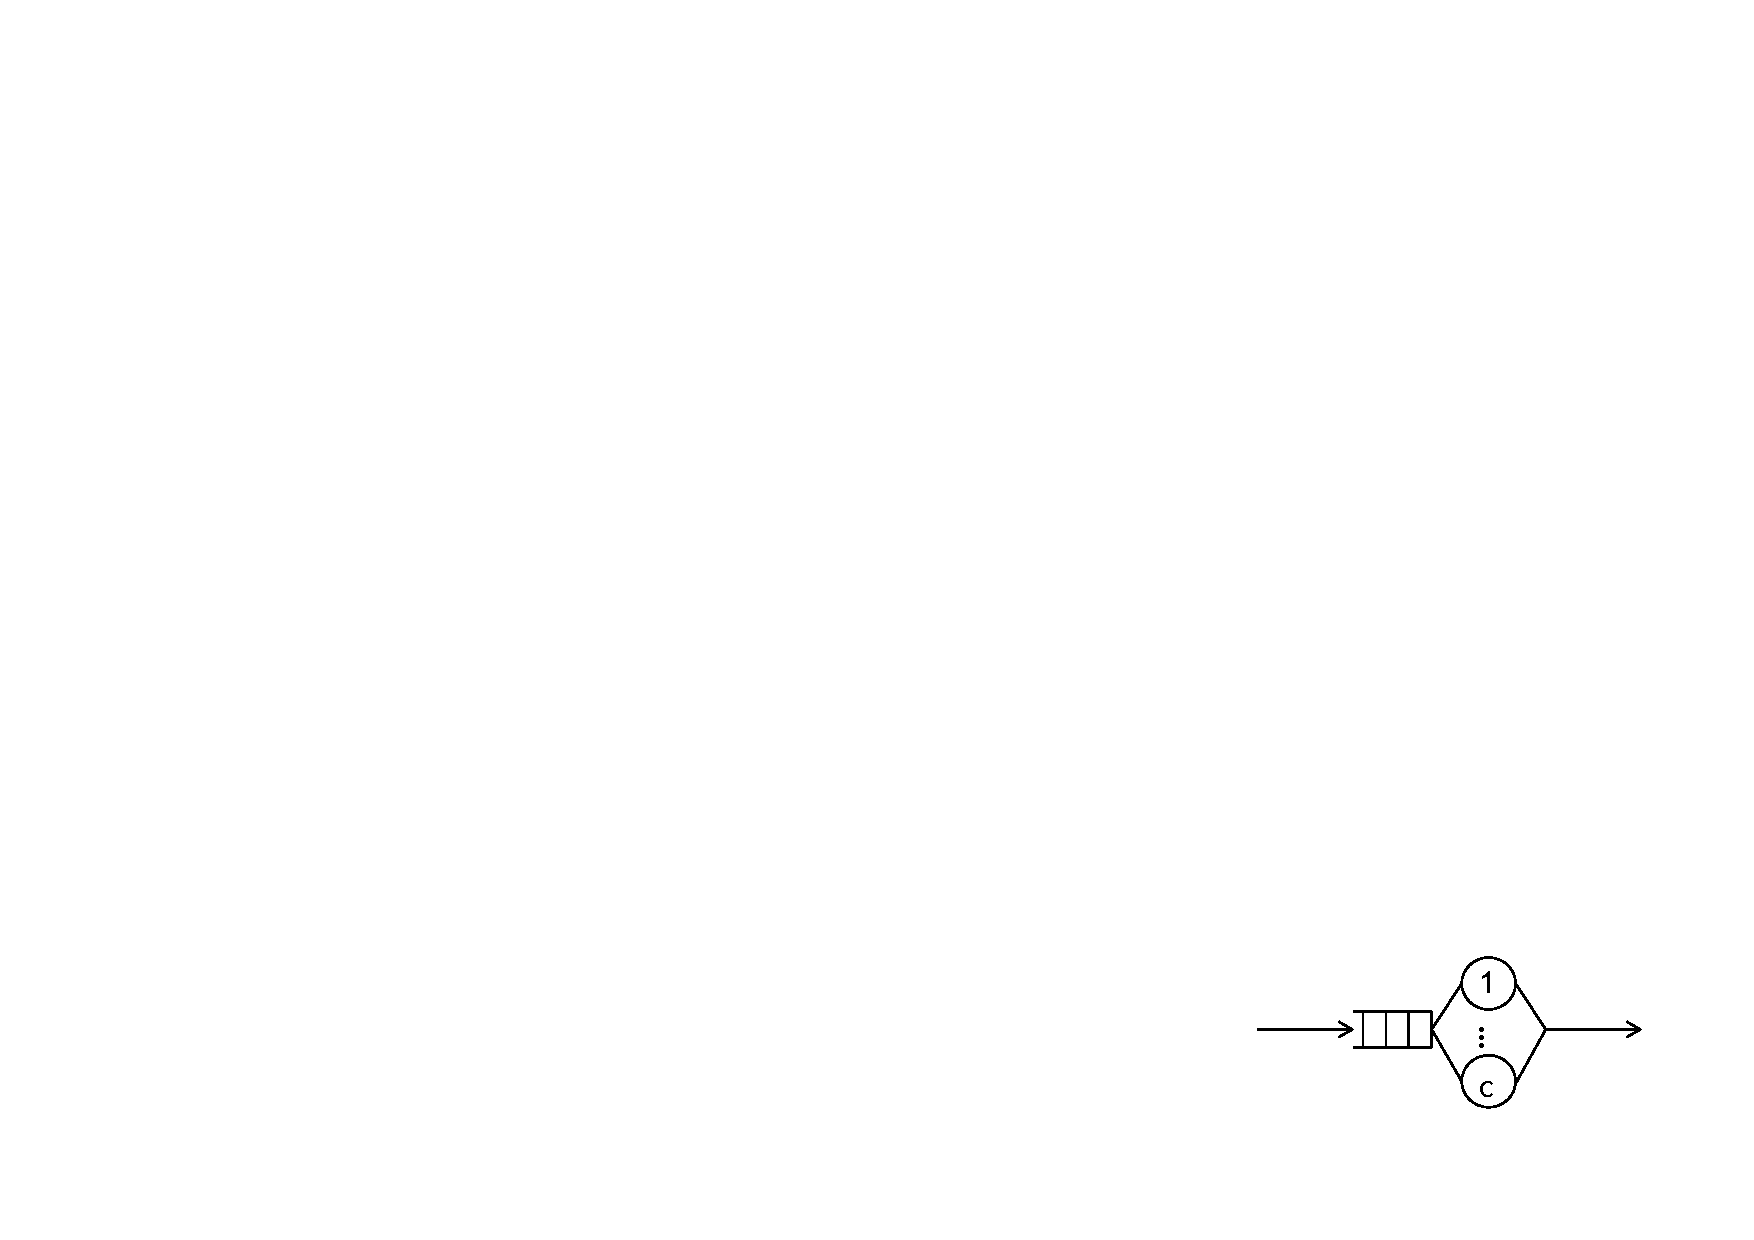
\includegraphics[width=.3\textwidth]{img/queueing-network-7.pdf}
		\end{figure}
	\end{itemize}
	
	\item \textbf{\underline{Queue}}. If \textbf{jobs exceed the parallel processing capacity of the system}, they are \textbf{forced to wait in a buffer}.
	
	When the job currently in service leaves the system, one of the jobs in the queue can now enter the free service center.
	\definition{Service Discipline}/\definition{Queuing Policy} \textbf{determines which of the jobs in the queue will be selected to start its service}.
	
	\item \textbf{\underline{Population}}. Ideally, members of the population are indistinguishable from one another. When this is not the case, we divide the population into \textbf{classes whose members all exhibit the same behavior}. Different classes differ in one or more characteristics, e.g. arrival rate, service demand. Identifying different classes is a task of workload characterization.
	
	\item \textbf{\underline{Routing}}. For many systems, we can view the system as a collection of resources and devices, with customers or jobs circulating between them.
	
	We can associate a service center with each resource in the system and then route customers between the service centers.
	
	After being serviced at one service center, a customer can move on to other service centers, following a pre-defined pattern of behavior according to the customer's needs.
	
	A queueing network can then be represented as a graph where the nodes represent the service centers k and the arcs represent the possible transitions of users from one service center to another. Nodes and arcs together define the network topology.
	
	Whenever \textbf{a job has several possible alternative routes after completing service at a station}, an appropriate selection policy must be defined.
	
	The policy is also called the \definition{Routing Algorithm}. The most important routing algorithms are:
	\begin{itemize}
		\item \definition{Probabilistic Routing Algorithm}. \textbf{Each path is assigned a probability of being chosen by the job that left the station in question}.
		
		\item \definition{Round Robin Routing Algorithm}. The \textbf{destination chosen by the job rotates among all possible existing destinations}.
		
		\item \definition{Join the shortest queue Routing Algorithm}. \textbf{Jobs can query the queue length of the possible destinations and choose the one with the least number of jobs waiting to be served}.
	\end{itemize}
\end{itemize}
With important definition of routing, we can say that a \textbf{network} can be:
\begin{itemize}
	\item \textbf{\underline{Open}}. Customers can come from or go to any external environment.
	\item \textbf{\underline{Closed}}. A fixed population of customers remains within the system.
	\item \textbf{\underline{Mixed}}. There are classes of customers within the system that exhibit both open and closed patterns of behavior.
\end{itemize}
An additional graphical notation is:
\begin{figure}[!htp]
	\centering
	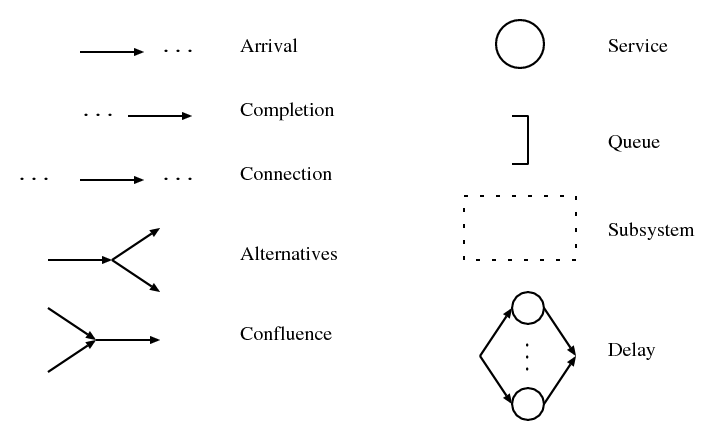
\includegraphics[width=\textwidth]{img/queueing-network-8.png}
\end{figure}

\begin{examplebox}[: Open Networks]
	A client server system, dealing with external arrivals (classical three tier architecture).
	
	Provide a QN model of the system and evaluate the overall throughput considering that the network delay is negligible with respect to the other devices and two different cases:
	\begin{enumerate}
		\item The only thing we know is that each server should be visited by the application.
		\item In the second case we know that the application \textbf{after visiting the web server} requires some operations at \textbf{the application server} and then \textbf{can go back} to \textbf{the web server} and \textbf{leave} the system \textbf{or} can require service at the \textbf{DMBS} and then \textbf{go back} to the \textbf{application server}.
	\end{enumerate}
	\begin{center}
		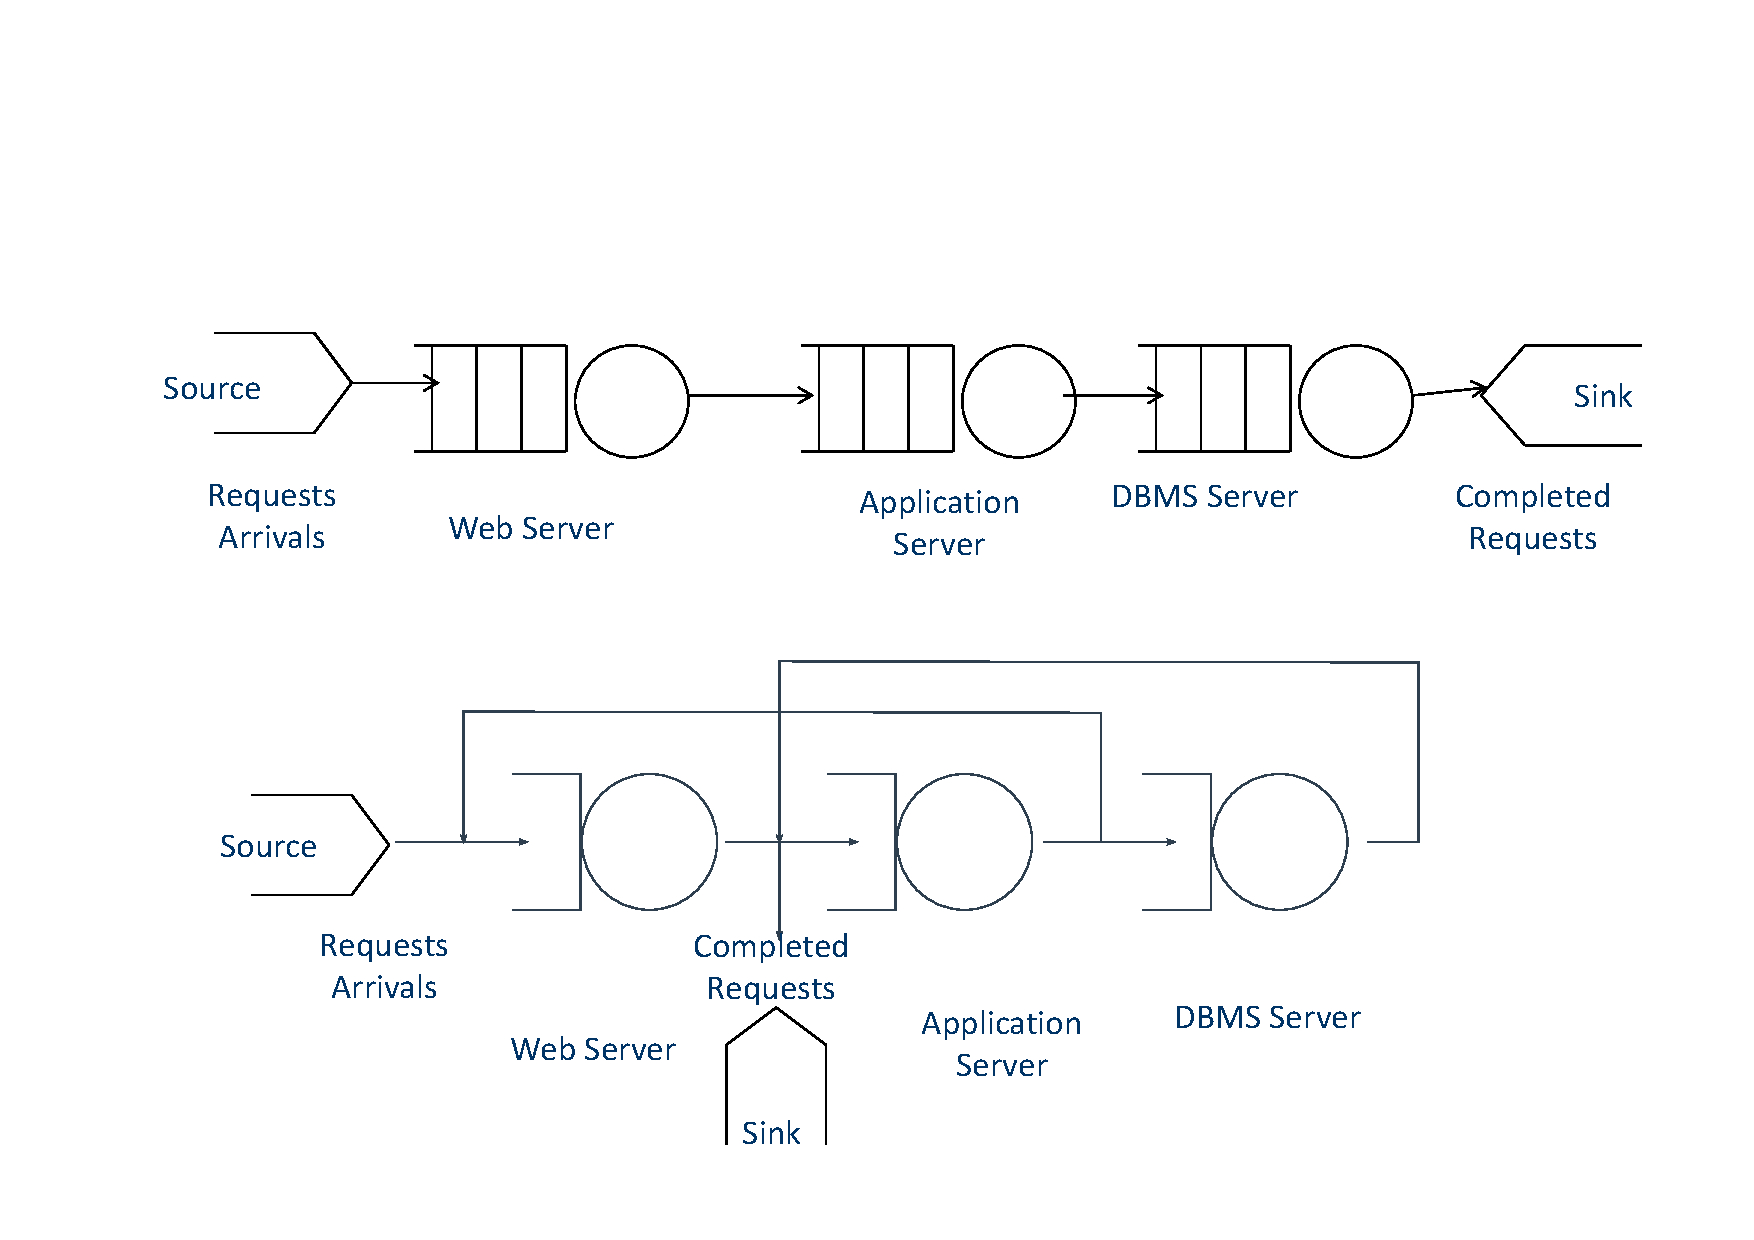
\includegraphics[width=\textwidth]{img/queueing-network-9.pdf}
	\end{center}
\end{examplebox}

\begin{examplebox}[: Closed Networks]
	A client server system, \textbf{with a finite number of customers} (classical three tier architecture and not accessible from outside).
	
	Provide a QN model of the system and evaluate the system throughput considering that Network delay is negligible with respect to the other devices. Model the two different cases previously described.
	\begin{itemize}
		\item First scenario
		\begin{center}
			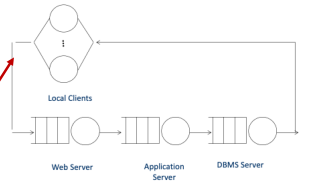
\includegraphics[width=.65\textwidth]{img/queueing-network-10.png}
		\end{center}
		
		\item Second scenario
		\begin{center}
			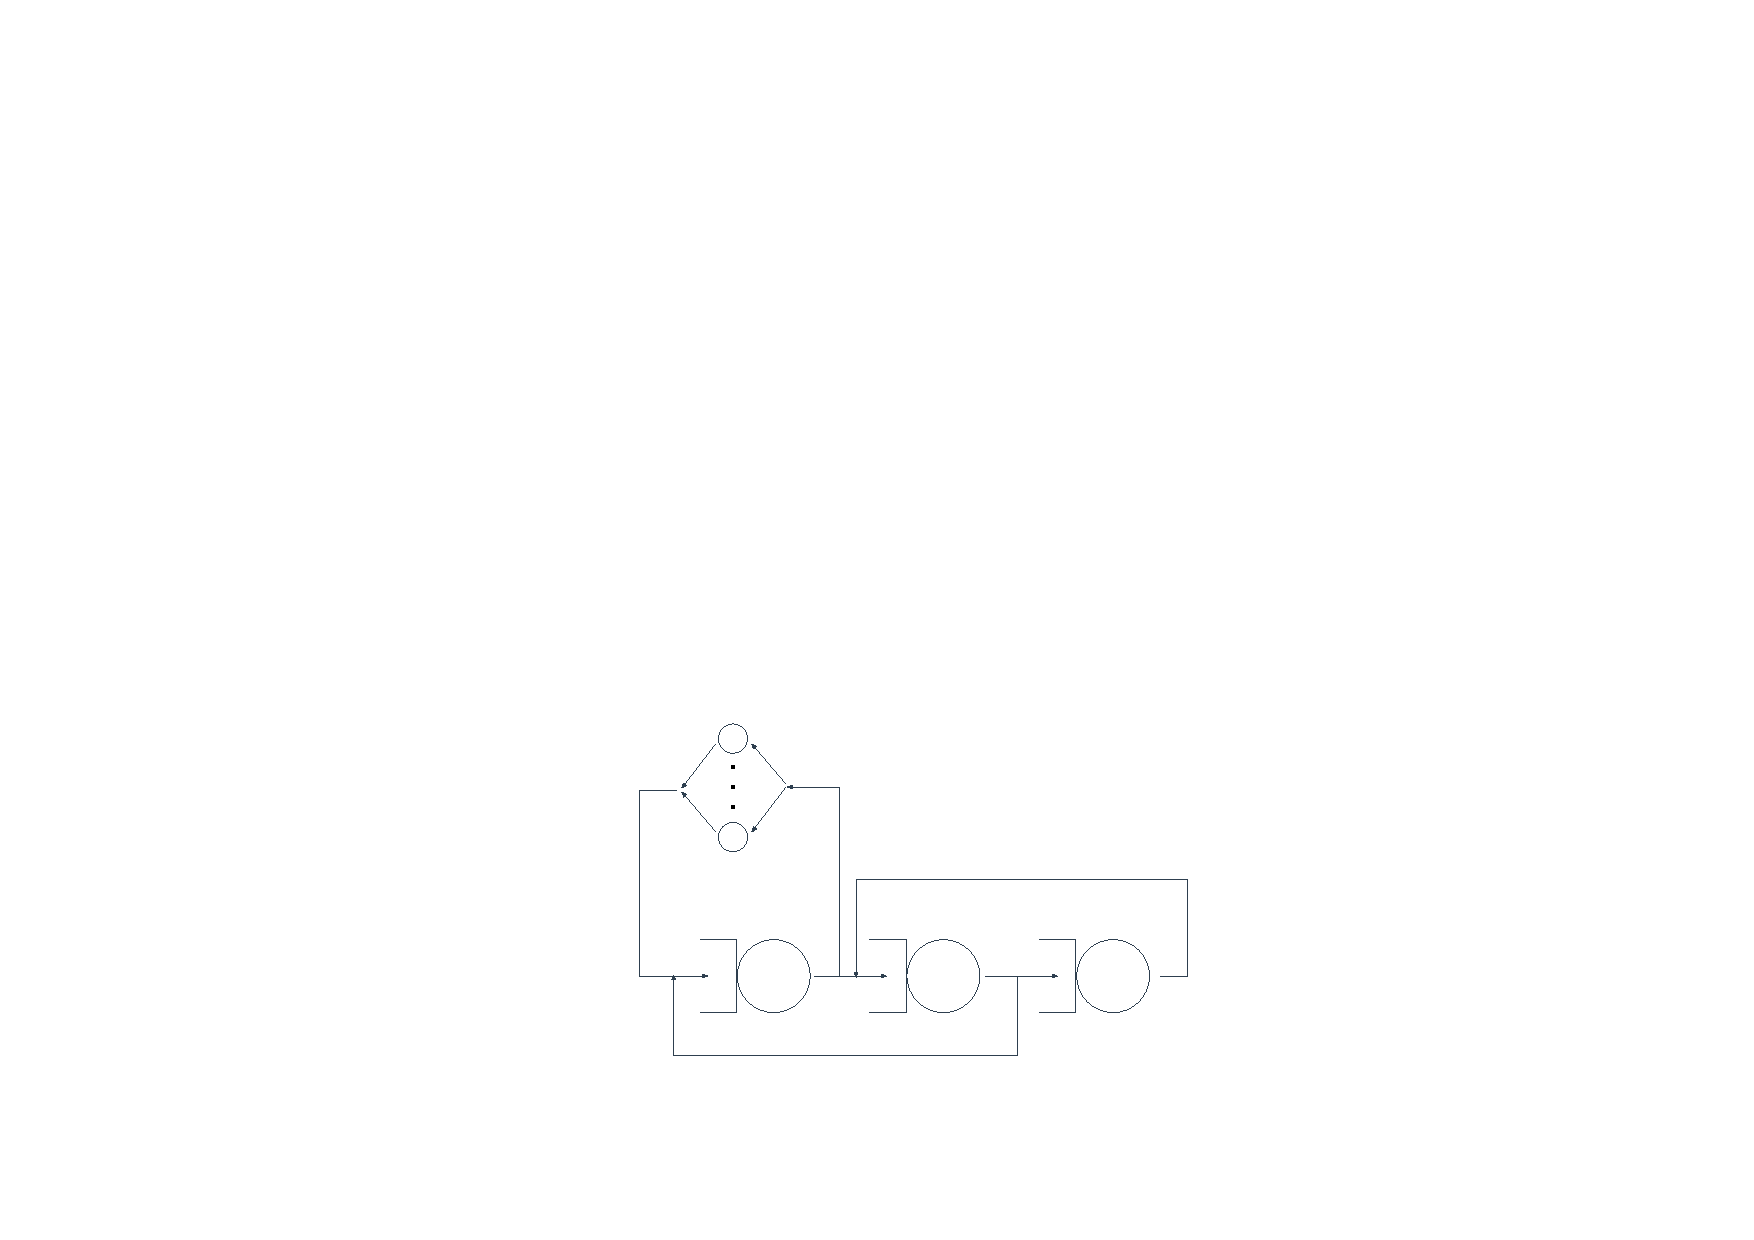
\includegraphics[width=.6\textwidth]{img/queueing-network-11.pdf}
		\end{center}
	\end{itemize}
\end{examplebox}

\newpage

\subsubsection{Operational Laws}

\definition{Operational Laws} are \textbf{simple equations} that can be \textbf{used as an abstract representation} or \textbf{model} of the average \textbf{behavior} of almost any \textbf{system}.

\begin{flushleft}
	\textcolor{Green3}{\faIcon{check-circle} \textbf{Advantages}}
\end{flushleft}
\begin{itemize}
	\item The laws are very \textbf{general} and make almost \textbf{no assumptions about the behavior of the random variables} that characterize the system.
	\item \textbf{Simplicity}: they can be applied quickly and easily.
\end{itemize}
In the Computing Infrastructure course, then in this note, the operational laws are applied to the Queueing Network model (\ref{subsubsection: Queueing Networks}, page \pageref{subsubsection: Queueing Networks}).

\highspace
Operational laws are based on \textbf{observable variables}, \textbf{values} that we can \textbf{derive by observing a system} over a finite period of time.

\highspace
In general, we assume that the \textbf{system receives requests from its environment}. Each \textbf{request creates a job} or \textbf{customer} within the system. Finally, when a job has been processed, the \textbf{system responds to the environment by completing the corresponding request}.

\longline

\paragraph{Basic measurements}

From an abstract system we can derive the following quantities:
\begin{itemize}
	\item \textbf{T}, the \textbf{length of time} we observe the system
	\item \textbf{A}, the number of request \textbf{arrivals} we observe
	\item \textbf{C}, the number of request \textbf{completions} we observe
	\item \textbf{B}, the total amount of time during which the system is \textbf{busy} ($B \le T$)
	\item \textbf{N}, the average \textbf{number of jobs} in the system
\end{itemize}
From these values, we can derive the following four important \textbf{quantities}:
\begin{itemize}
	\item \definition{Arrival rate}:
	\begin{equation}
		\lambda = \dfrac{\text{number of request arrivals}}{\text{length of time we observe the system}} = \dfrac{A}{T}
	\end{equation}
	
	\item \definition{Throughput} or \definition{Completion rate}:
	\begin{equation}
		X = \dfrac{\text{number of request completions}}{\text{length of time we observe the system}} = \dfrac{C}{T}
	\end{equation}
	
	\item \definition{Utilization}:
	\begin{equation}
		U = \dfrac{\text{total amount of time during which the system is busy}}{\text{length of time we observe the system}} = \dfrac{B}{T}
	\end{equation}
	
	\item \definition{Mean service time} per completed job:
	\begin{equation}
		S = \dfrac{\text{total amount of time during which the system is busy}}{\text{number of request completions}} = \dfrac{B}{C}
	\end{equation}
\end{itemize}
We will assume that the \textbf{system is job-flow balanced}. Then the \textbf{number of arrivals is equal to the number of completions} during an observation period.

\highspace
Note that if the system is job flow balanced, then the \textbf{arrival rate is equal to the completion rate (throughput)}:
\begin{equation*}
	\lambda = X
\end{equation*}

\highspace
A \textbf{system} can be thought of as \textbf{consisting} of a number of devices or \textbf{resources}. Each of these can be treated as a \textbf{separate system} from the perspective of operational laws.

\highspace
An \textbf{external request generates a job} within the system; this job may \textbf{then circulate among the resources} until all the necessary processing has been done; as it arrives at each resource, it is treated as a request, generating a job internal to that resource.

\highspace
In this case, we have the following quantities:
\begin{itemize}
	\item \textbf{T}, the \textbf{length of time} we observe the system
	\item $\mathbf{A}_{k}$, the number of request \textbf{arrivals} we observe for resource $k$
	\item $\mathbf{C}_{k}$, the number of request \textbf{completions} we observe at resource $k$
	\item $\mathbf{B}_{k}$, the total amount of time during which the resource $k$ is \textbf{busy} ($B_{k} \le T$)
	\item $\mathbf{N}_{k}$, the average \textbf{number of jobs} in the resource $k$
\end{itemize}
And we can derive the following four quantities for resource k:
\begin{itemize}
	\item \definition{Arrival rate}:
	\begin{equation}
		\lambda_{k} = \dfrac{A_{k}}{T}
	\end{equation}
	
	\item \definition{Throughput} or \definition{Completion rate}:
	\begin{equation}
		X_{k} = \dfrac{C_{k}}{T}
	\end{equation}
	
	\item \definition{Utilization}:
	\begin{equation}
		U_{k} = \dfrac{B_{k}}{T}
	\end{equation}
	
	\item \definition{Mean service time} per completed job:
	\begin{equation}
		S_{k} = \dfrac{B_{k}}{C_{k}}
	\end{equation}
\end{itemize}

\newpage

\paragraph{Utilization Law}

Using the formulas:
\begin{itemize}
	\item Throughput: $X_{k} = \dfrac{C_{k}}{T}$
	\item Mean service time: $S_{k} = \dfrac{B_{k}}{C_{k}}$
	\item Utilization: $U_{k} = \dfrac{B_{k}}{T}$
\end{itemize}
From:
\begin{equation*}
	X_{k} \cdot S_{k} = \dfrac{C_{k}}{T} \cdot \dfrac{B_{k}}{C_{k}} = \dfrac{B_{k}}{T} = U_{k}
\end{equation*}
We can derive the \definition{Utilization Law}:
\begin{equation}
	U_{k} = X_{k} \cdot S_{k}
\end{equation}

\longline

\paragraph{Little's Law}

The \definition{Little's Law} is:
\begin{equation}
	N = X \cdot R
\end{equation}
In other words, $N$ is equal to the \textbf{number of requests in the system}. Little's Law can be applied to the entire system as well as to some subsystems.

\highspace
If the system throughput is $X$ requests/sec, and each request remains in the system on average for $R$ seconds, then for each unit of time, we can observe on average $XR$ requests in the system.

\begin{examplebox}
	Consider a disk that serves 40 requests/seconds ($X = 40$ req/s) and suppose that on average there are $4$ requests ($N=4$) present in the disk system (waiting to be served or in service).
	
	Little's Law tell that $N = XR \Rightarrow R = \frac{N}{X}$, so the average time spent at the disk by a request must be $\frac{4}{40} = 0.1$.
	
	If we know $S$ (e.g.) each request requires 0.0225 seconds of disk service and we can then deduce that the average waiting time (time in the queue) is 0.0775 seconds.
\end{examplebox}
The value of Little's Law changes depending on the application:
\begin{itemize}
	\item \textbf{\underline{Service level}}.
	\begin{itemize}
		\item The service time is:
		\begin{equation*}
			R = S
		\end{equation*}
		Where $R$ is the average of each request remaining in the system.
		\item The utilization is:
		\begin{equation*}
			N = X \cdot R = X \cdot S = U
		\end{equation*}
	\end{itemize}
	\begin{figure}[!htp]
		\centering
		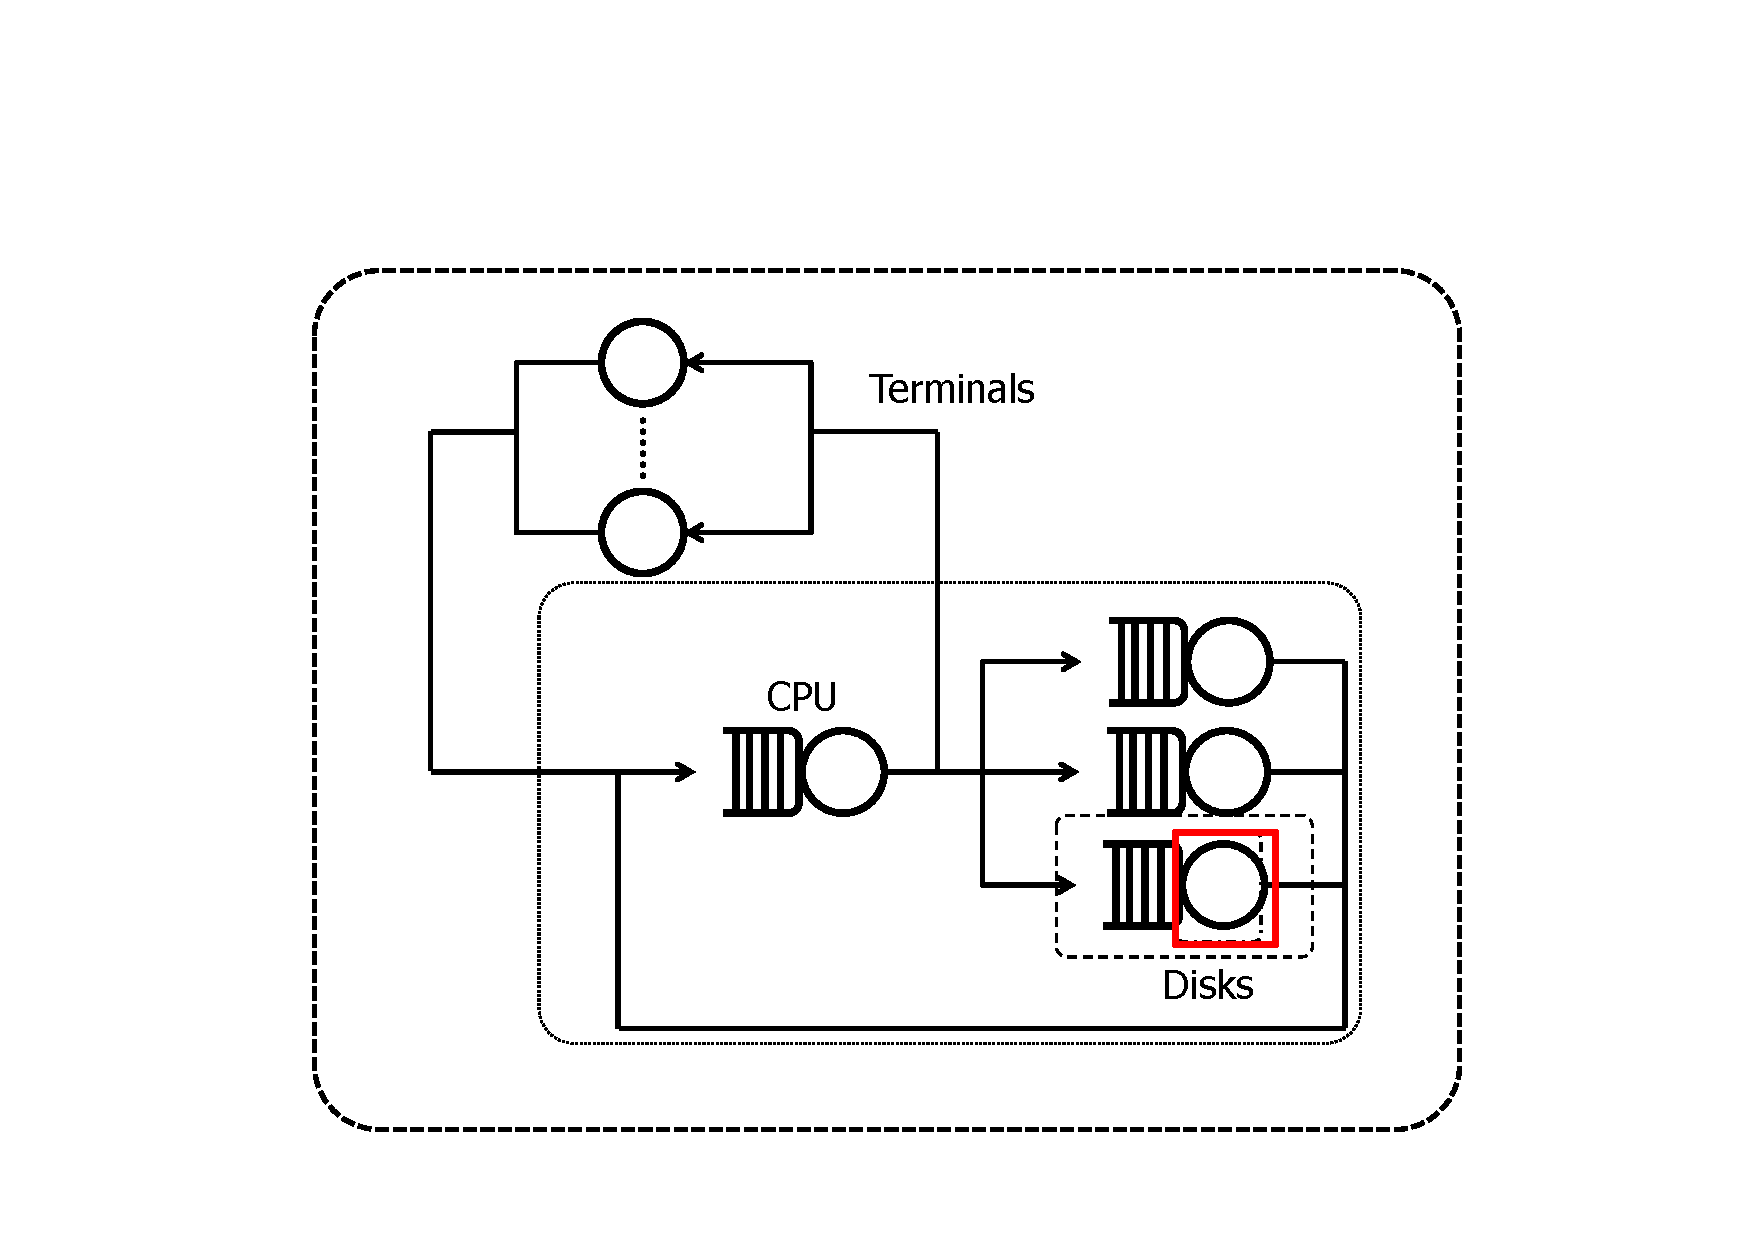
\includegraphics[width=.7\textwidth]{img/little-law-1.pdf}
	\end{figure}
	
	\item \textbf{\underline{Service and Queue level}}. 
	\begin{itemize}
		\item The service time is:
		\begin{equation*}
			R = S
		\end{equation*}
		Where $R$ is the average of each request remaining in the system.
		\item The utilization is:
		\begin{equation*}
			N = \text{Flying requests} \Rightarrow \dfrac{N}{X} = R = \left(S + T_{\text{queue}}\right)
		\end{equation*}
	\end{itemize}
	\begin{figure}[!htp]
		\centering
		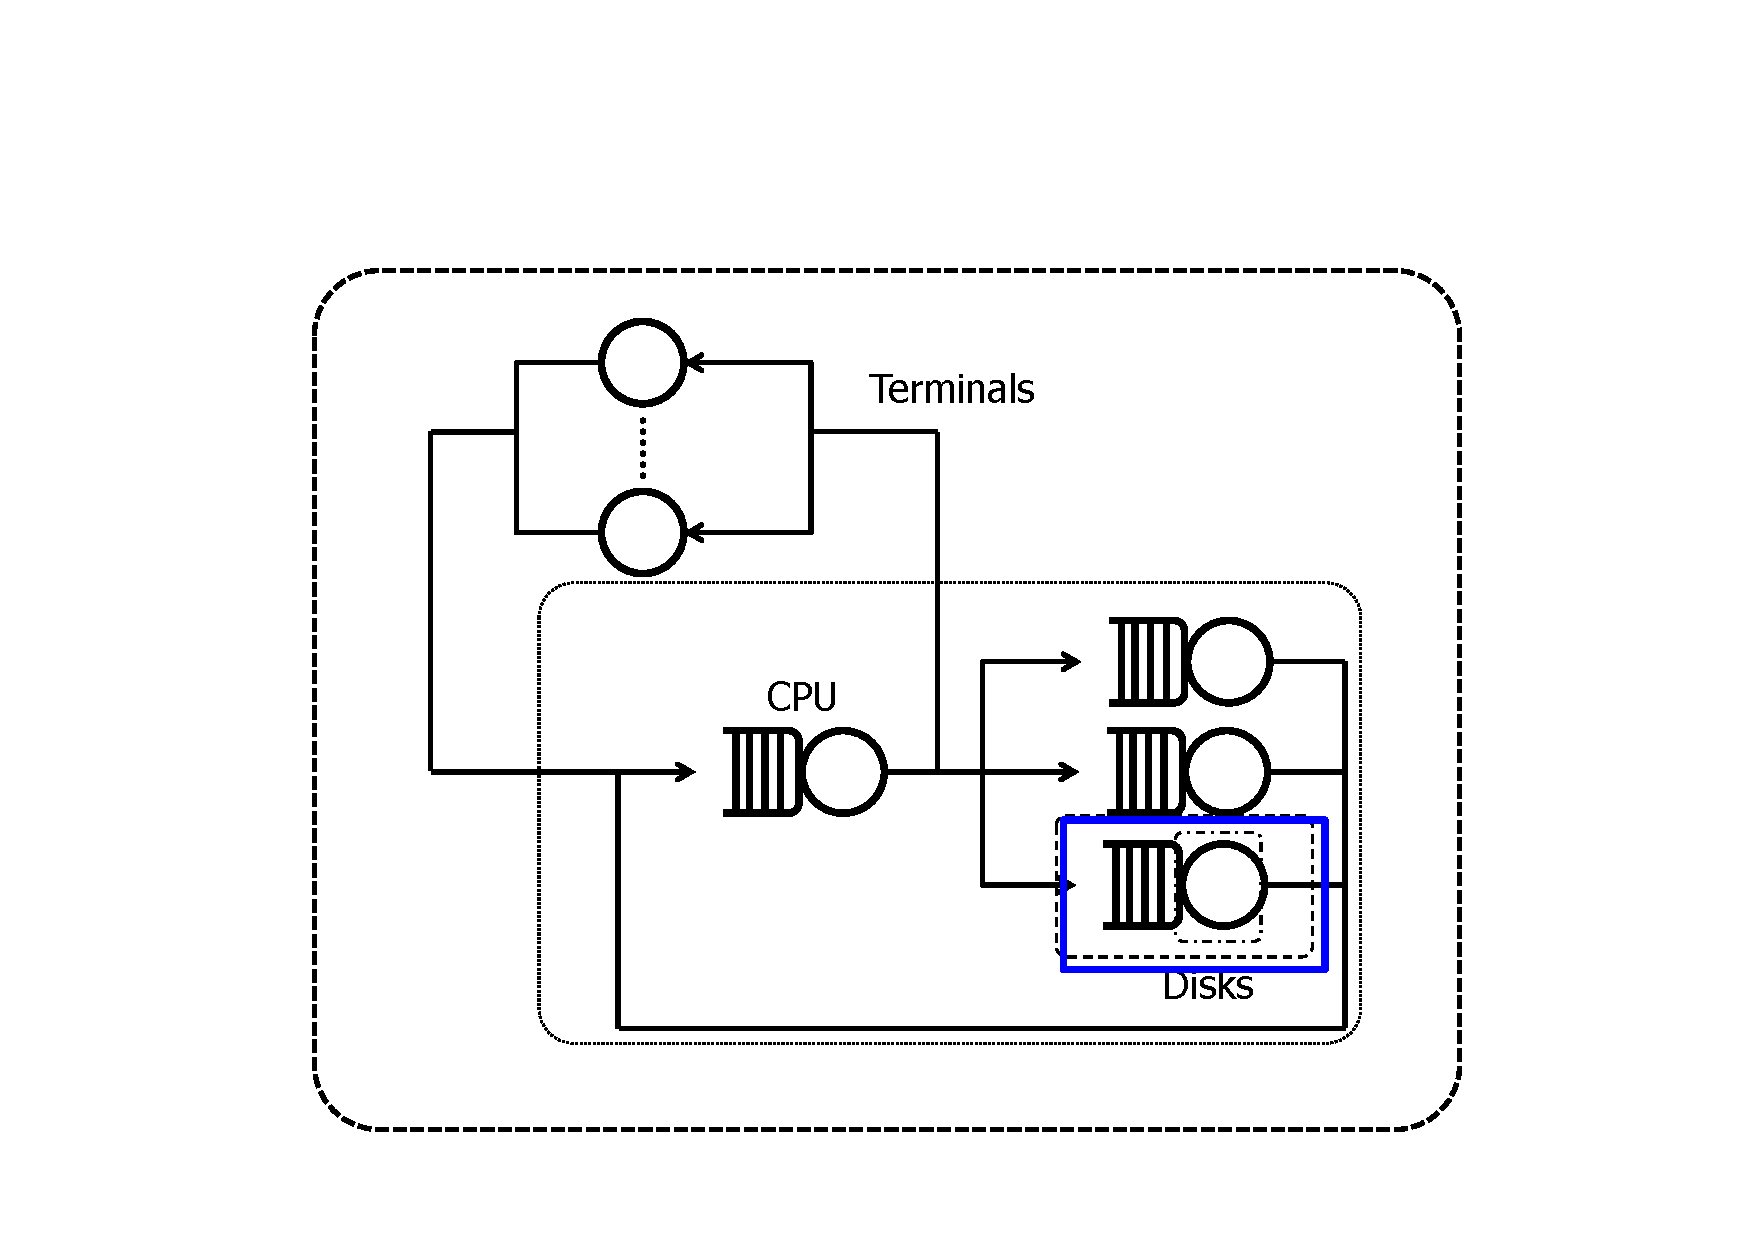
\includegraphics[width=.7\textwidth]{img/little-law-2.pdf}
	\end{figure}
	
	\item \textbf{\underline{Subsystem level}}. 
	\begin{itemize}
		\item The service time is:
		\begin{equation*}
			R = \text{Residence Time}
		\end{equation*}
		Residence time corresponds to our conventional notion of response time: the period of time from when a user submits a request until that user's response is returned.
		\item The utilization is:
		\begin{equation*}
			N = \text{Flying requests} \Rightarrow \dfrac{N}{X} = R
		\end{equation*}
	\end{itemize}
	\begin{figure}[!htp]
		\centering
		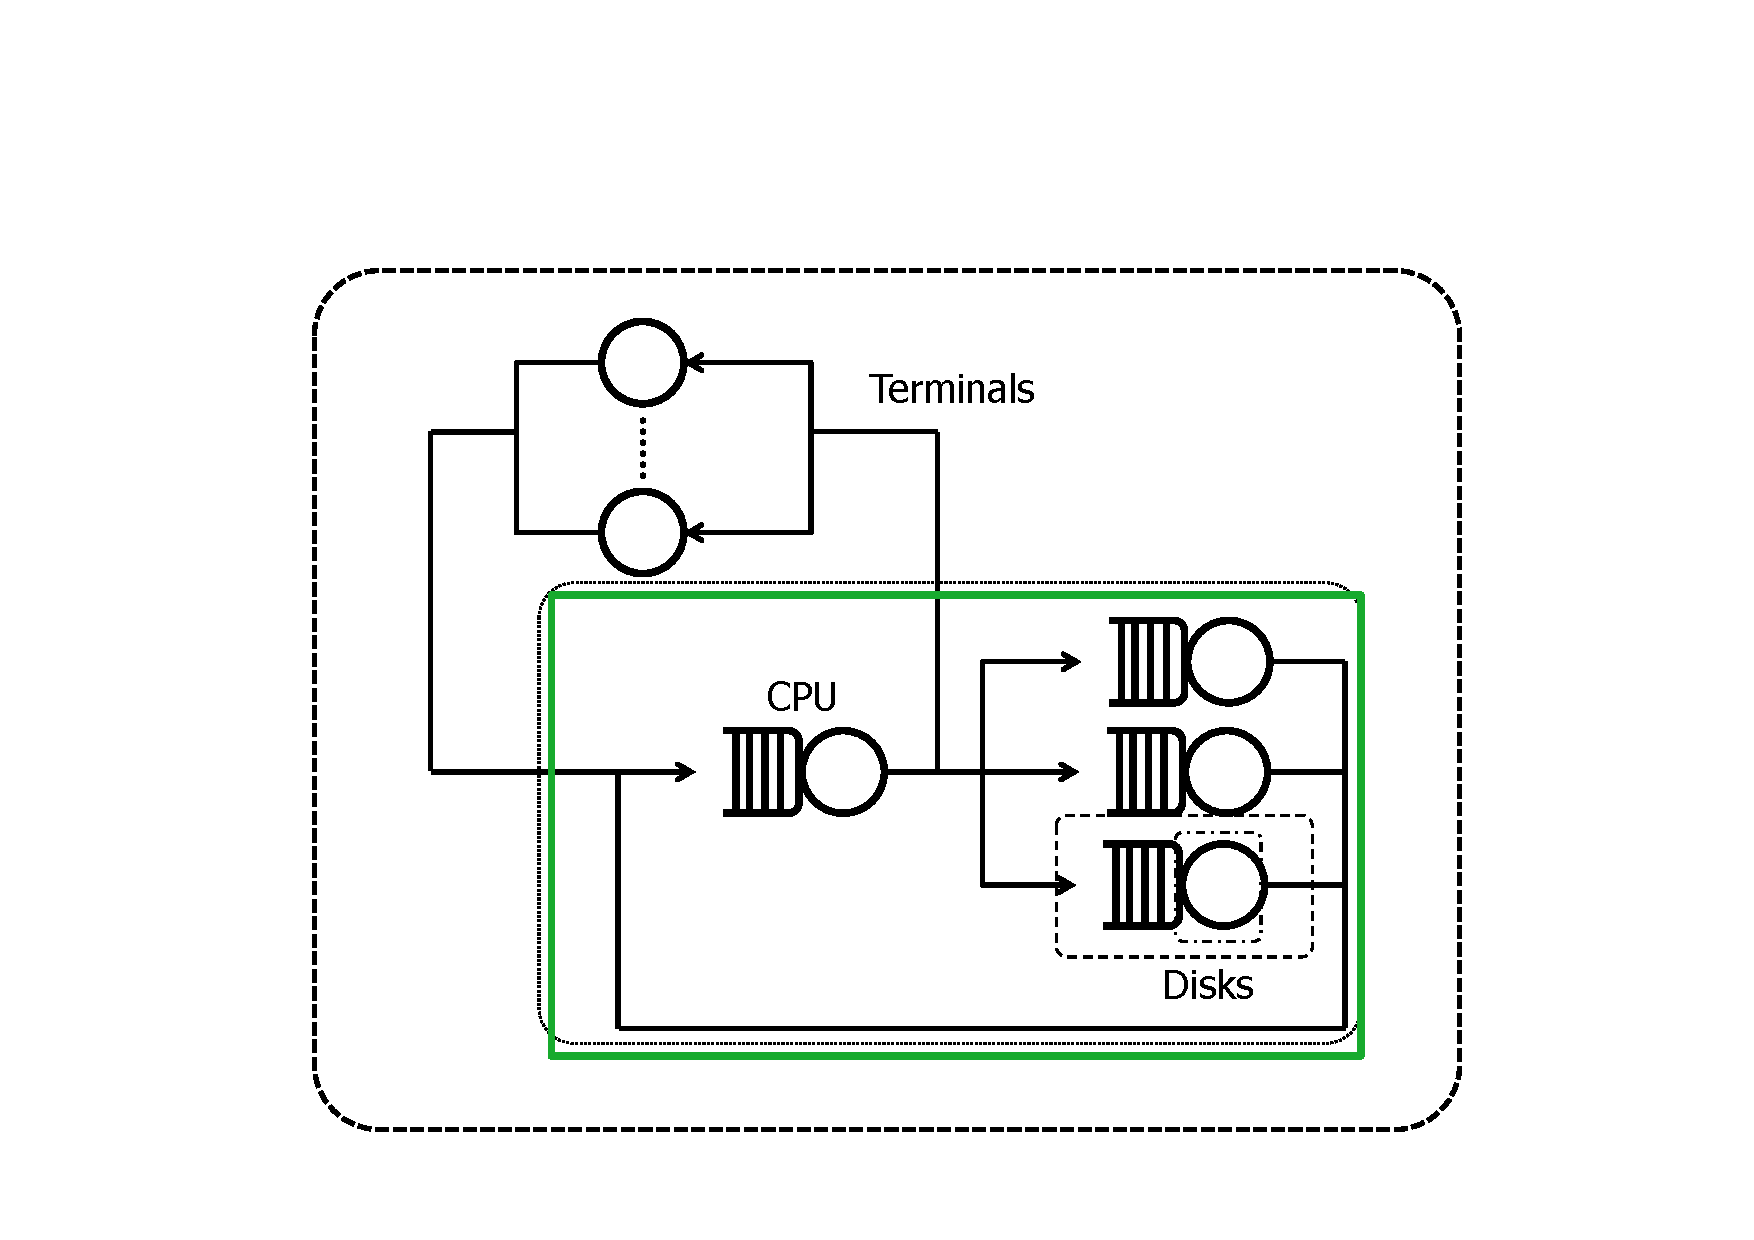
\includegraphics[width=.7\textwidth]{img/little-law-3.pdf}
	\end{figure}
	
	\item \textbf{\underline{System level}}. 
	\begin{figure}[!htp]
		\centering
		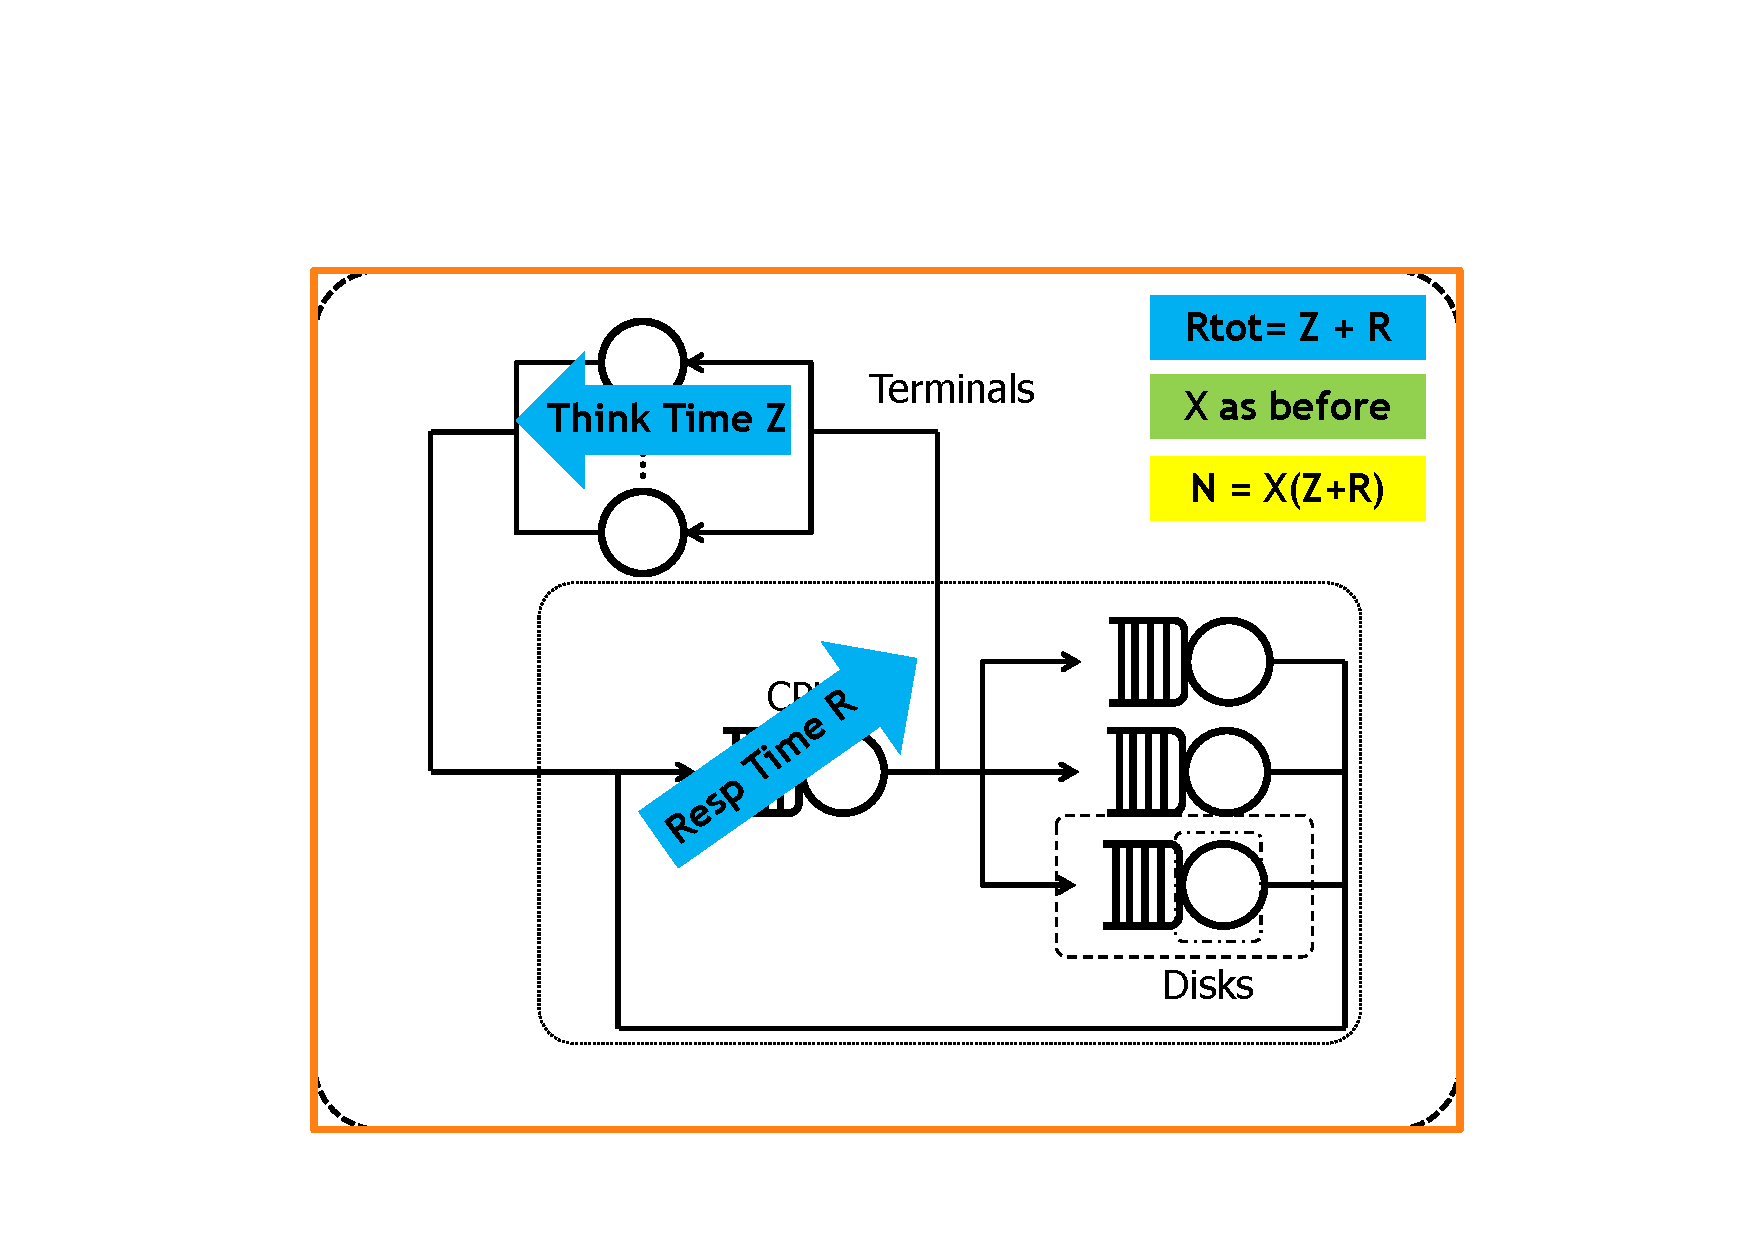
\includegraphics[width=.7\textwidth]{img/little-law-4.pdf}
	\end{figure}
\end{itemize}

\newpage

\paragraph{Interactive Response Time Law}

The \definition{Interactive Response Time Law} is:
\begin{equation}
	R = \dfrac{N}{X} - Z
\end{equation}
The response time in an interactive system is the \textbf{residence time minus the think time}. Note that \textbf{if the think time is zero} ($Z=0$) and $R = \frac{N}{X}$, then the \textbf{interactive response time law simply becomes Little's Law}.

\begin{examplebox}
	Suppose that the library catalogue system has \textbf{64 interactive users} connected via Browsers, the average \textbf{think time is 30 seconds}, and that system \textbf{throughput is 2 interactions/second}. What is the response time?
	
	The interactive response time law tell us that the response time must be $\dfrac{64}{2}-30 = 2$ seconds.
\end{examplebox}

\longline

\paragraph{Visit count}

In an observation interval we can count not only completions external to the system, but also the number of completions at each resource within the system. We denote $C_{k}$ by the \textbf{number of completions at resource} $k$. We define the \definition{Visit Count}:
\begin{equation}
	V_{k} = \dfrac{C_{k}}{C}
\end{equation}
It is the ratio of the number of completions at the $k$-th resource to the number of system completions.

\begin{examplebox}
	If, during an observation interval, we measure \textbf{10 system completions} and \textbf{150 completions at a specific disk}, then on average each system-level request requires \textbf{15 disk operations}.
\end{examplebox}

\noindent
Note that:
\begin{itemize}
	\item If \underline{$C_{k} > C$}, resource $k$ is \textbf{visited several times} (on average) during each system level request. This happens when there are \textbf{loops in the model}.
	
	\item If \underline{$C_{k} < C$}, resource $k$ \textbf{might not be visited} during each system level request. This can happen if there are \textbf{alternatives} (e.g. caching of disks).
	
	\item If \underline{$C_{k} = C$}, resource $k$ is \textbf{visited} (on average) \textbf{exactly once every request}.
\end{itemize}

\newpage

\paragraph{Forced Flow Law}

The \definition{Forced Flow Law} captures the \textbf{relationship between the different components within a system}. It states that the throughputs, or flows, in all parts of a system must be proportional to each other.
\begin{equation}
	X_{k} = V_{k} \cdot X
\end{equation}
The throughput at the $k$-th resource is equal to the product of the throughput of the system and the visit count at that resource.

\highspace
Rewriting $C_{k} = V_{k} \cdot C$ and applying $X_{k} = \frac{C_{k}}{T}$, we can derive the forced flow law:
\begin{equation*}
	C_{k} = V_{k} \cdot C \: \Rightarrow \: \dfrac{C_{k}}{T} = \dfrac{V_{k} \cdot C}{T} \: \Rightarrow \: X_{k} = V_{k} \cdot X
\end{equation*}

\longline

\paragraph{Utilization Law with Service Demand}

If we know the amount of processing each job requires at a resource then we can calculate the utilization of the resource.

\highspace
Let us assume that each time a job visits the $k$-th resource, the amount of processing or service time it requires is $S_{k}$.

\highspace
Note that \textbf{service time is not the same as the residence time} of the job at that resource. In general a job might have to \textbf{wait} for some time \textbf{before processing} being.

\highspace
The \textbf{total amount of service that a system job generates at the $k$-th resource} is called the \definition{Service Demand $D_{k}$}:
\begin{equation}
	D_{k} = S_{k} \cdot V_{k}
\end{equation}
Using the service demand, we can rewrite the \definition{Utilization Law}:
\begin{equation}
	U_{k} = X_{k} \cdot S_{k} = \left(X \cdot V_{k}\right) \cdot S_{k} = D_{k} \cdot X
\end{equation}
The utilization of a resource is denoted $U_{k}$ and it is the percentage of time that the $k$-th resource is in use processing a job. It is also equal to the product of:
\begin{itemize}
	\item The throughput of that resource and the average service time at that resource;
	
	\item The throughput at system level and the average service demand at that resource.
\end{itemize}

\newpage

\paragraph{Response and Residence Times}

When considering nodes characterized by visits different from one, we can define two permanence times: Response Time and Residence Time.

\highspace
The \definition{Response Time $\tilde{R}_{k}$} (or $\Phi_{k}$) accounts for the \textbf{average time spent in station} $k$, when the \textbf{job enters the corresponding node} (i.e. time for the single interaction, disk request):
\begin{figure}[!htp]
	\centering
	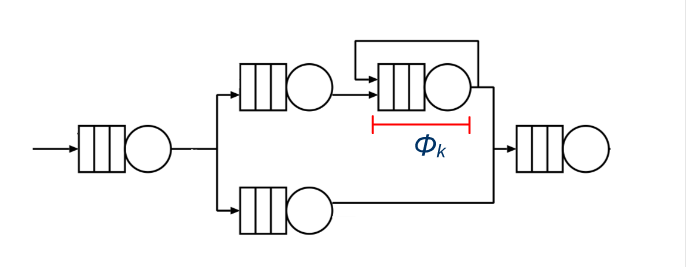
\includegraphics[width=0.7\textwidth]{img/response-time.png}
\end{figure}

\noindent
The \definition{Residence Time $R_{k}$} accounts instead for the \textbf{average time spent by a job at station $k$ during the staying in the system}: it can be greater or smaller than the response time depending on the number of visits.
\begin{figure}[!htp]
	\centering
	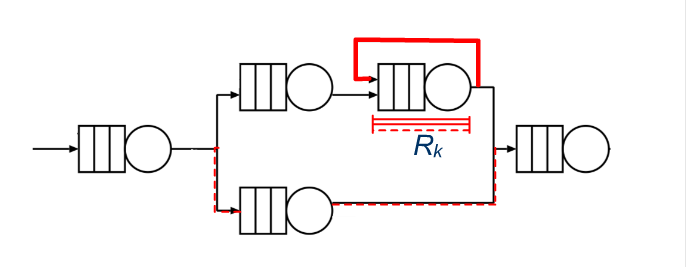
\includegraphics[width=0.7\textwidth]{img/residence-time.png}
\end{figure}

\noindent
Note that there is the same relation between Residence Time and Response Time as the one between \definition{Demand Time} and \definition{Service Time}:
\begin{equation}
	\begin{array}{rcl}
		D_{k} &=& v_{k} \cdot S_{k} \\ [.3em]
		R_{k} &=& v_{k} \cdot \tilde{R}_{k}
	\end{array}
\end{equation}
Also note that for \textbf{single queue open system}, or \emph{tandem models}, $v_{k} = 1$. This implies that \textbf{average service time and service demand are equal, and response time and residence time are identical}.
\begin{equation*}
	v_{k} = 1 \Rightarrow
	\begin{array}{rcl}
		D_{k} &=& S_{k} \\ [.3em]
		R_{k} &=& \tilde{R}_{k}
	\end{array}
\end{equation*}